\documentclass[12pt,a4paper]{article}
\usepackage[utf8]{inputenc}
\usepackage[T1]{fontenc}
\usepackage[english,indonesian]{babel}
\usepackage{times}
\usepackage{amsmath}
\usepackage{amsfonts}
\usepackage{amssymb}
\usepackage{graphicx}
\usepackage{longtable}
\usepackage{hyperref}
\usepackage{geometry}
\geometry{top=2.5cm, left=2.5cm, bottom=2.5cm, right=2.5cm}
\usepackage{titlesec}
\usepackage{multicol}

\usepackage{fancyhdr}
% \setlength{\headheight}{56pt}
\setlength{\footskip}{34pt}
\pagestyle{plain}
\sloppy

\titleformat{\section}{\normalfont\fontsize{12}{14}\bfseries}{\thesection}{1em}{}
\titleformat{\subsection}{\normalfont\fontsize{12}{14}\bfseries}{\thesubsection}{1em}{}
\titleformat{\subsubsection}{\normalfont\fontsize{12}{14}\bfseries}{\thesubsubsection}{1em}{}

\title{
{\fontsize{16}{19}\selectfont\bfseries Agentic AI Untuk Tata Kelola Data Kearsipan Konsisten Dan Terstruktur}
\vspace{10pt} \\
{\fontsize{16}{19}\selectfont\bfseries Achieving Consistency And Structure In Archival Data Governance Through Agentic AI}
}
\author{Jatniko Nur Mutaqin \\ \\ Arsip Nasional Republik Indonesia \\ Email: jatnikonm@anri.go.id}
\date{}

\begin{document}

% Ensure title is rendered and page style is plain for the title page
\maketitle
	hispagestyle{plain}
\begin{abstract}
\normalsize
\centering
\textbf{Abstrak}

Tata kelola kearsipan konvensional menghadapi tantangan inkonsistensi kebijakan, metadata tidak terstruktur, dan penegakan aturan yang tidak konsisten. Penelitian ini merancang model konseptual berbasis \emph{Agentic AI} untuk mengatasi masalah tersebut secara sistematis. Menggunakan pendekatan \emph{Design Science Research} (DSR), penelitian menghasilkan arsitektur Sistem Multi-Agen (MAS) holistik yang terdiri dari agen-agen cerdas otonom dan terspesialisasi (Agen Klasifikasi, Agen Metadata, Agen Kepatuhan), dikoordinasikan oleh agen orkestrator. Hasil menunjukkan pendekatan ini mengubah paradigma tata kelola dari kebijakan pasif menjadi logika aktif terintegrasi, dimana aturan kearsipan dieksekusi secara otonom dan konsisten. Implementasi model diproyeksikan meningkatkan konsistensi proses, kualitas metadata, dan pencapaian Indikator Kinerja Utama (IKU) kearsipan secara objektif dan terukur.

\textbf{Kata Kunci}: \emph{Agentic AI}, Sistem Multi-Agen, Tata Kelola Data, Kearsipan Digital
\end{abstract}

\selectlanguage{english}
\renewcommand{\abstractname}{}

\begin{abstract}
\normalsize
\centering
\textbf{Abstract}

Conventional archival data governance faces critical challenges including inconsistent policy implementation, unstructured metadata, and difficulties in maintaining consistent rule enforcement across organizational units. These issues significantly impact operational efficiency, compliance, and the achievement of Key Performance Indicators (KPIs). This research addresses these challenges by designing and proposing a conceptual model based on Agentic AI to systematically transform archival data governance. Employing a Design Science Research (DSR) approach, this study develops a comprehensive Multi-Agent System (MAS) architecture comprising autonomous, specialized intelligent agents---including Classification Agent, Metadata Agent, and Compliance Agent---coordinated by an orchestrator agent. The primary contribution of this research reveals that the proposed approach fundamentally shifts the governance paradigm from passive policy documents to active, integrated operational logic, where archival rules and standards are autonomously and consistently executed by AI agents. The implementation of this model is projected to significantly enhance process consistency, improve metadata quality and structure, and support more objective and measurable achievement of archival KPIs. This research contributes both theoretical frameworks for understanding AI-driven governance automation and practical architectural guidance for archival institutions.

\textbf{Keywords}: Agentic AI, Multi-Agent System, Data Governance, Digital Archives
\end{abstract}

\clearpage
\begin{multicols}{2}

\section{PENDAHULUAN}

\subsection{Latar Belakang}

Tata kelola data kearsipan yang efektif merupakan komponen fundamental bagi operasional, akuntabilitas, dan keberlanjutan organisasi modern (Maurel and Zwarich 2021). Berbagai studi dan praktik terbaik di bidang manajemen informasi secara konsisten menekankan bahwa pengelolaan arsip yang baik tidak hanya krusial untuk mendukung pengambilan keputusan strategis berbasis bukti (Luo and Hu 2022; Tummers, Kassahun, and Tekinerdogan 2020) dan memastikan kepatuhan terhadap kerangka regulasi hukum yang berlaku (Christiana, Helminasari, and Pratama 2024; Kerpedzhiev et al. 2020), tetapi juga vital dalam melestarikan memori kolektif serta aset intelektual organisasi (Colavizza et al. 2021). 

Meskipun demikian, implementasi tata kelola kearsipan yang optimal menghadapi berbagai tantangan (Ma 2024; Liu 2024), terutama dalam sistem yang masih mengandalkan proses manual atau semi-otomatis. Masalah yang kerap diidentifikasi dalam literatur meliputi: (1) inkonsistensi dalam penerapan kebijakan dan prosedur kearsipan antar unit kerja (Miller et al. 2020), yang berakibat pada pengelolaan arsip yang tidak seragam dan sulit diaudit; (2) kesulitan dalam menjaga metadata arsip agar tetap terstruktur, lengkap, dan akurat secara konsisten (Jones et al. 2023), padahal metadata berkualitas tinggi merupakan prasyarat penting untuk temu kembali informasi yang efisien; dan (3) lambatnya proses pencarian dan akses terhadap arsip (Indrasweri, Dwi Wahyuni, and Rakhmawati 2022), yang berpotensi menghambat produktivitas organisasi. Standar dan kebijakan yang jelas merupakan kunci untuk interoperabilitas (Magnuson, Merrick, and Case 2020), namun penerapan konsisten di lapangan masih menjadi tantangan.

Berbagai tantangan ini dapat berdampak pada kesulitan organisasi dalam mencapai target Indikator Kinerja Utama (IKU) (Luo and Hu 2022; Tripathi, Agrawal, and Gupta 2020). Dalam konteks ini, perkembangan teknologi Kecerdasan Artifisial (AI), khususnya paradigma \emph{Agentic AI}, mulai dieksplorasi sebagai pendekatan yang berpotensi memberikan solusi signifikan. \emph{Agentic AI}, dengan karakteristiknya yang otonom, proaktif, dan adaptif (Hosseini and Seilani 2025; Sapkota, Roumeliotis, and Karkee 2025), membuka peluang untuk merepresentasikan berbagai fungsi krusial dalam tata kelola data kearsipan---mulai dari akuisisi, klasifikasi otomatis, manajemen metadata cerdas (Shinde et al. 2024), hingga pemantauan kepatuhan terhadap kebijakan---sebagai serangkaian agen AI yang bekerja terkoordinasi. Dengan mendelegasikan tugas-tugas yang terdefinisi dengan baik dan repetitif kepada agen-agen AI (Masimov and Hajiyev 2024), diharapkan dapat tercapai tingkat konsistensi yang lebih tinggi dalam penerapan kebijakan dan menghasilkan struktur metadata yang lebih berkualitas.

\subsection{Pertanyaan Penelitian}

Menyadari potensi transformatif \emph{Agentic AI} dan mengidentifikasi celah dalam penelitian terkini, penelitian ini dirumuskan untuk menjawab pertanyaan fundamental berikut:

\begin{enumerate}
\item Bagaimana arsitektur sistem berbasis \emph{Agentic AI} dapat dirancang secara optimal untuk merepresentasikan dan melaksanakan tugas-tugas kunci dalam tata kelola data kearsipan, dengan fokus pada peningkatan konsistensi penerapan kebijakan dan perbaikan struktur metadata?

\item Sejauh mana integrasi \emph{Agentic AI} berpotensi memberikan kontribusi terhadap pencapaian IKU kearsipan yang lebih objektif dan terukur?

\item Apa saja faktor-faktor kritis---termasuk tantangan implementasi praktis (Sapkota, Roumeliotis, and Karkee 2025), kebutuhan supervisi manusia, dan aspek integrasi---yang perlu dipertimbangkan untuk memastikan efektivitas dan akuntabilitas (Ackerman 2025; Raza et al. 2025) sistem \emph{Agentic AI} dalam tata kelola data kearsipan?
\end{enumerate}

\subsection{Tujuan Penelitian}

Sejalan dengan pertanyaan penelitian, penelitian ini menetapkan tujuan spesifik sebagai berikut:

\begin{enumerate}
\item Merancang dan mengusulkan model konseptual arsitektur sistem berbasis \emph{Agentic AI} yang mampu merepresentasikan dan mengotomatisasi tugas-tugas kunci dalam siklus hidup arsip dan proses tata kelola, sehingga berkontribusi pada peningkatan konsistensi penerapan kebijakan dan kualitas struktur metadata.

\item Menganalisis dan memetakan secara komprehensif potensi kontribusi implementasi \emph{Agentic AI} terhadap peningkatan objektivitas dalam pengukuran dan pencapaian IKU di bidang kearsipan.

\item Mengidentifikasi dan mengevaluasi secara kritis faktor-faktor pendukung dan penghambat---mencakup aspek teknis, organisasional, serta kebutuhan intervensi manusia dalam skema \emph{human-in-the-loop}---guna memastikan penerapan \emph{Agentic AI} yang efektif dan akuntabel.
\end{enumerate}

\subsection{Manfaat Penelitian}

Penelitian ini diharapkan memberikan manfaat yang signifikan baik dari perspektif teoritis maupun praktis.

\textbf{Manfaat Teoritis:} Penelitian ini berpotensi memperkaya khazanah ilmu pengetahuan dalam disiplin manajemen informasi, ilmu kearsipan, dan kecerdasan artifisial, terutama terkait aplikasi inovatif \emph{Agentic AI} dalam konteks tata kelola data. Penelitian ini juga menyediakan kerangka kerja konseptual baru untuk memahami bagaimana tugas-tugas kompleks dalam tata kelola kearsipan dapat direpresentasikan dan diotomatisasi secara efektif melalui arsitektur sistem berbasis agen AI.

\textbf{Manfaat Praktis:} Penelitian ini menyediakan panduan dan model arsitektur yang dapat diadopsi oleh institusi kearsipan dalam merancang dan mengimplementasikan solusi \emph{Agentic AI} untuk meningkatkan efisiensi operasional, konsistensi pengelolaan, dan kualitas data kearsipan. Penelitian ini juga menawarkan wawasan bagi pengambil keputusan dan praktisi kearsipan mengenai potensi \emph{Agentic AI} dalam mendukung pencapaian IKU dan meningkatkan akuntabilitas. Dengan mengidentifikasi faktor-faktor kunci yang perlu diperhatikan, penelitian ini membantu meminimalkan risiko dan memaksimalkan dampak positif dari adopsi teknologi AI di bidang kearsipan.

\section{KAJIAN PUSTAKA}

Literatur akademis dan standar industri secara konsisten menghadapi tantangan-tantangan dalam tata kelola arsip digital yang telah diuraikan pada bagian Pendahuluan. Untuk mengatasi tantangan tersebut, kerangka kerja seperti ISO 15489:2016 menjadi acuan fundamental yang menetapkan prinsip-prinsip untuk manajemen arsip yang akuntabel, termasuk penciptaan, penggunaan, pemeliharaan, dan disposisi arsip. Prinsip-prinsip ini menekankan pentingnya arsip yang otentik, andal, utuh, dan dapat digunakan. Namun, penerapan prinsip-prinsip ini secara konsisten di lingkungan digital yang kompleks dan bervolume besar tetap menjadi hambatan utama, yang mendorong perlunya eksplorasi solusi teknologi inovatif.

\subsection{Paradigma Agentic AI dan Sistem Multi-Agen (MAS)}

Untuk menjawab kebutuhan akan solusi yang lebih dinamis dan otonom, penelitian ini berfokus pada paradigma Agentic AI. Berbeda dengan AI konvensional yang reaktif, Agentic AI dirancang untuk bertindak secara proaktif dan adaptif guna mencapai tujuan yang kompleks. Arsitektur yang umum digunakan untuk implementasinya adalah Sistem Multi-Agen (MAS), di mana sistem terdiri dari beberapa agen cerdas yang berkolaborasi.

Menurut literatur teknis, arsitektur MAS yang efektif memiliki beberapa komponen kunci: (a) Agen-agen Spesialis: Entitas otonom yang memiliki keahlian khusus (misalnya, analisis data, validasi kepatuhan). (b) Agen Koordinator/Orkestrator: Pengatur alur kerja yang mendelegasikan tugas dan mengelola interaksi antar agen (c) Basis Pengetahuan Bersama: Repositori aturan, model, dan kebijakan yang dapat diakses oleh semua agen untuk memastikan konsistensi dalam pengambilan keputusan.

Pendekatan arsitektural ini telah terbukti berhasil mengotomatisasi proses kompleks di domain lain seperti keuangan dan logistik, dan menawarkan potensi besar untuk diterapkan pada tata kelola kearsipan.

\subsection{Peta Penelitian AI dalam Kearsipan dan Celah yang Ada}

Penerapan AI dalam ilmu kearsipan cenderung bersifat terpisah. Tinjauan sistematis dan studi kasus dari lembaga arsip menunjukkan bahwa AI lebih banyak digunakan sebagai alat untuk tugas-tugas spesifik (task-specific), seperti klasifikasi otomatis, ekstraksi metadata, atau dukungan akses informasi.

Meskipun penelitian terdahulu telah mengeksplorasi penggunaan agen untuk pelestarian digital, terdapat celah penelitian yang jelas: belum adanya model arsitektur terintegrasi yang menerapkan paradigma MAS modern untuk mengelola keseluruhan siklus hidup tata kelola kearsipan, mulai dari akuisisi hingga pemantauan IKU secara berkelanjutan. Penelitian ini dirancang untuk mengisi celah tersebut dengan mengusulkan model konseptual yang holistik.

\section{METODE PENELITIAN}

Penelitian ini menerapkan pendekatan Design Science Research (DSR) untuk menghasilkan artefak utama berupa model konseptual arsitektur Agentic AI. Fokus DSR dalam konteks ini adalah pada perancangan solusi inovatif untuk meningkatkan konsistensi dan struktur dalam tata kelola data kearsipan.

Pengembangan model ini didasarkan pada sintesis kritis dari sumber data sekunder yang komprehensif. Sumber utama meliputi: (1) Literatur ilmiah terkini (jurnal, prosiding, buku) mengenai tata kelola kearsipan, Agentic AI, Multi-Agent Systems, dan IKU kearsipan; (2) Standar internasional relevan (khususnya seri ISO 15489) dan dokumen kebijakan terkait; serta (3) Laporan praktik dan studi kasus publikasi mengenai implementasi sistem informasi atau AI di organisasi.

Pengumpulan data dilakukan melalui dua teknik utama: (1) Studi literatur sistematis terfokus untuk mengidentifikasi landasan teoritis, praktik terbaik, dan lanskap teknologi Agentic AI yang relevan; dan (2) Analisis dokumen kualitatif terhadap standar dan laporan untuk mengekstrak persyaratan fungsional, kriteria IKU, dan konteks implementasi.

Proses perancangan artefak model konseptual melibatkan identifikasi komponen agen AI kunci yang merepresentasikan fungsi tata kelola kearsipan, pendefinisian fungsionalitas dan interaksi antar agen, serta pemetaan alur kerja yang didukung oleh agen-agen tersebut. Prinsip-prinsip desain sistem cerdas dan tata kelola AI yang bertanggung jawab menjadi acuan dalam perancangan.

Evaluasi model konseptual dilakukan secara analitis dan kualitatif. Ini mencakup demonstrasi potensi model melalui skenario kasus penggunaan ilustratif, pemetaan model terhadap kriteria desain yang diturunkan dari literatur, serta analisis potensi kontribusinya terhadap IKU kearsipan dan identifikasi faktor-faktor implementasi kritis.

\section{HASIL DAN BAHASAN}

\subsection{Kapabilitas Agentic AI untuk Tata Kelola Kearsipan}

Transformasi tata kelola data kearsipan menuju sistem yang lebih konsisten, terstruktur, dan efisien dapat secara signifikan didukung oleh pemanfaatan kapabilitas kunci yang inheren dalam paradigma Agentic AI. Analisis mendalam mengidentifikasi beberapa kapabilitas fundamental yang paling relevan dan berpotensi memberikan dampak transformatif, yang akan diuraikan sebagai berikut:

\subsubsection{Otonomi Terarah}

Deskripsi Kapabilitas: Agen AI dirancang untuk beroperasi secara mandiri dalam batas-batas dan tujuan yang telah ditetapkan oleh manusia (arsiparis atau administrator sistem). Agen ini dapat menjalankan serangkaian tugas tanpa intervensi langsung untuk setiap langkah, namun tetap bekerja menuju sasaran spesifik yang telah dikonfigurasikan, seperti penerapan skema klasifikasi atau validasi kelengkapan metadata.

\begin{figure}[htbp]
\centering
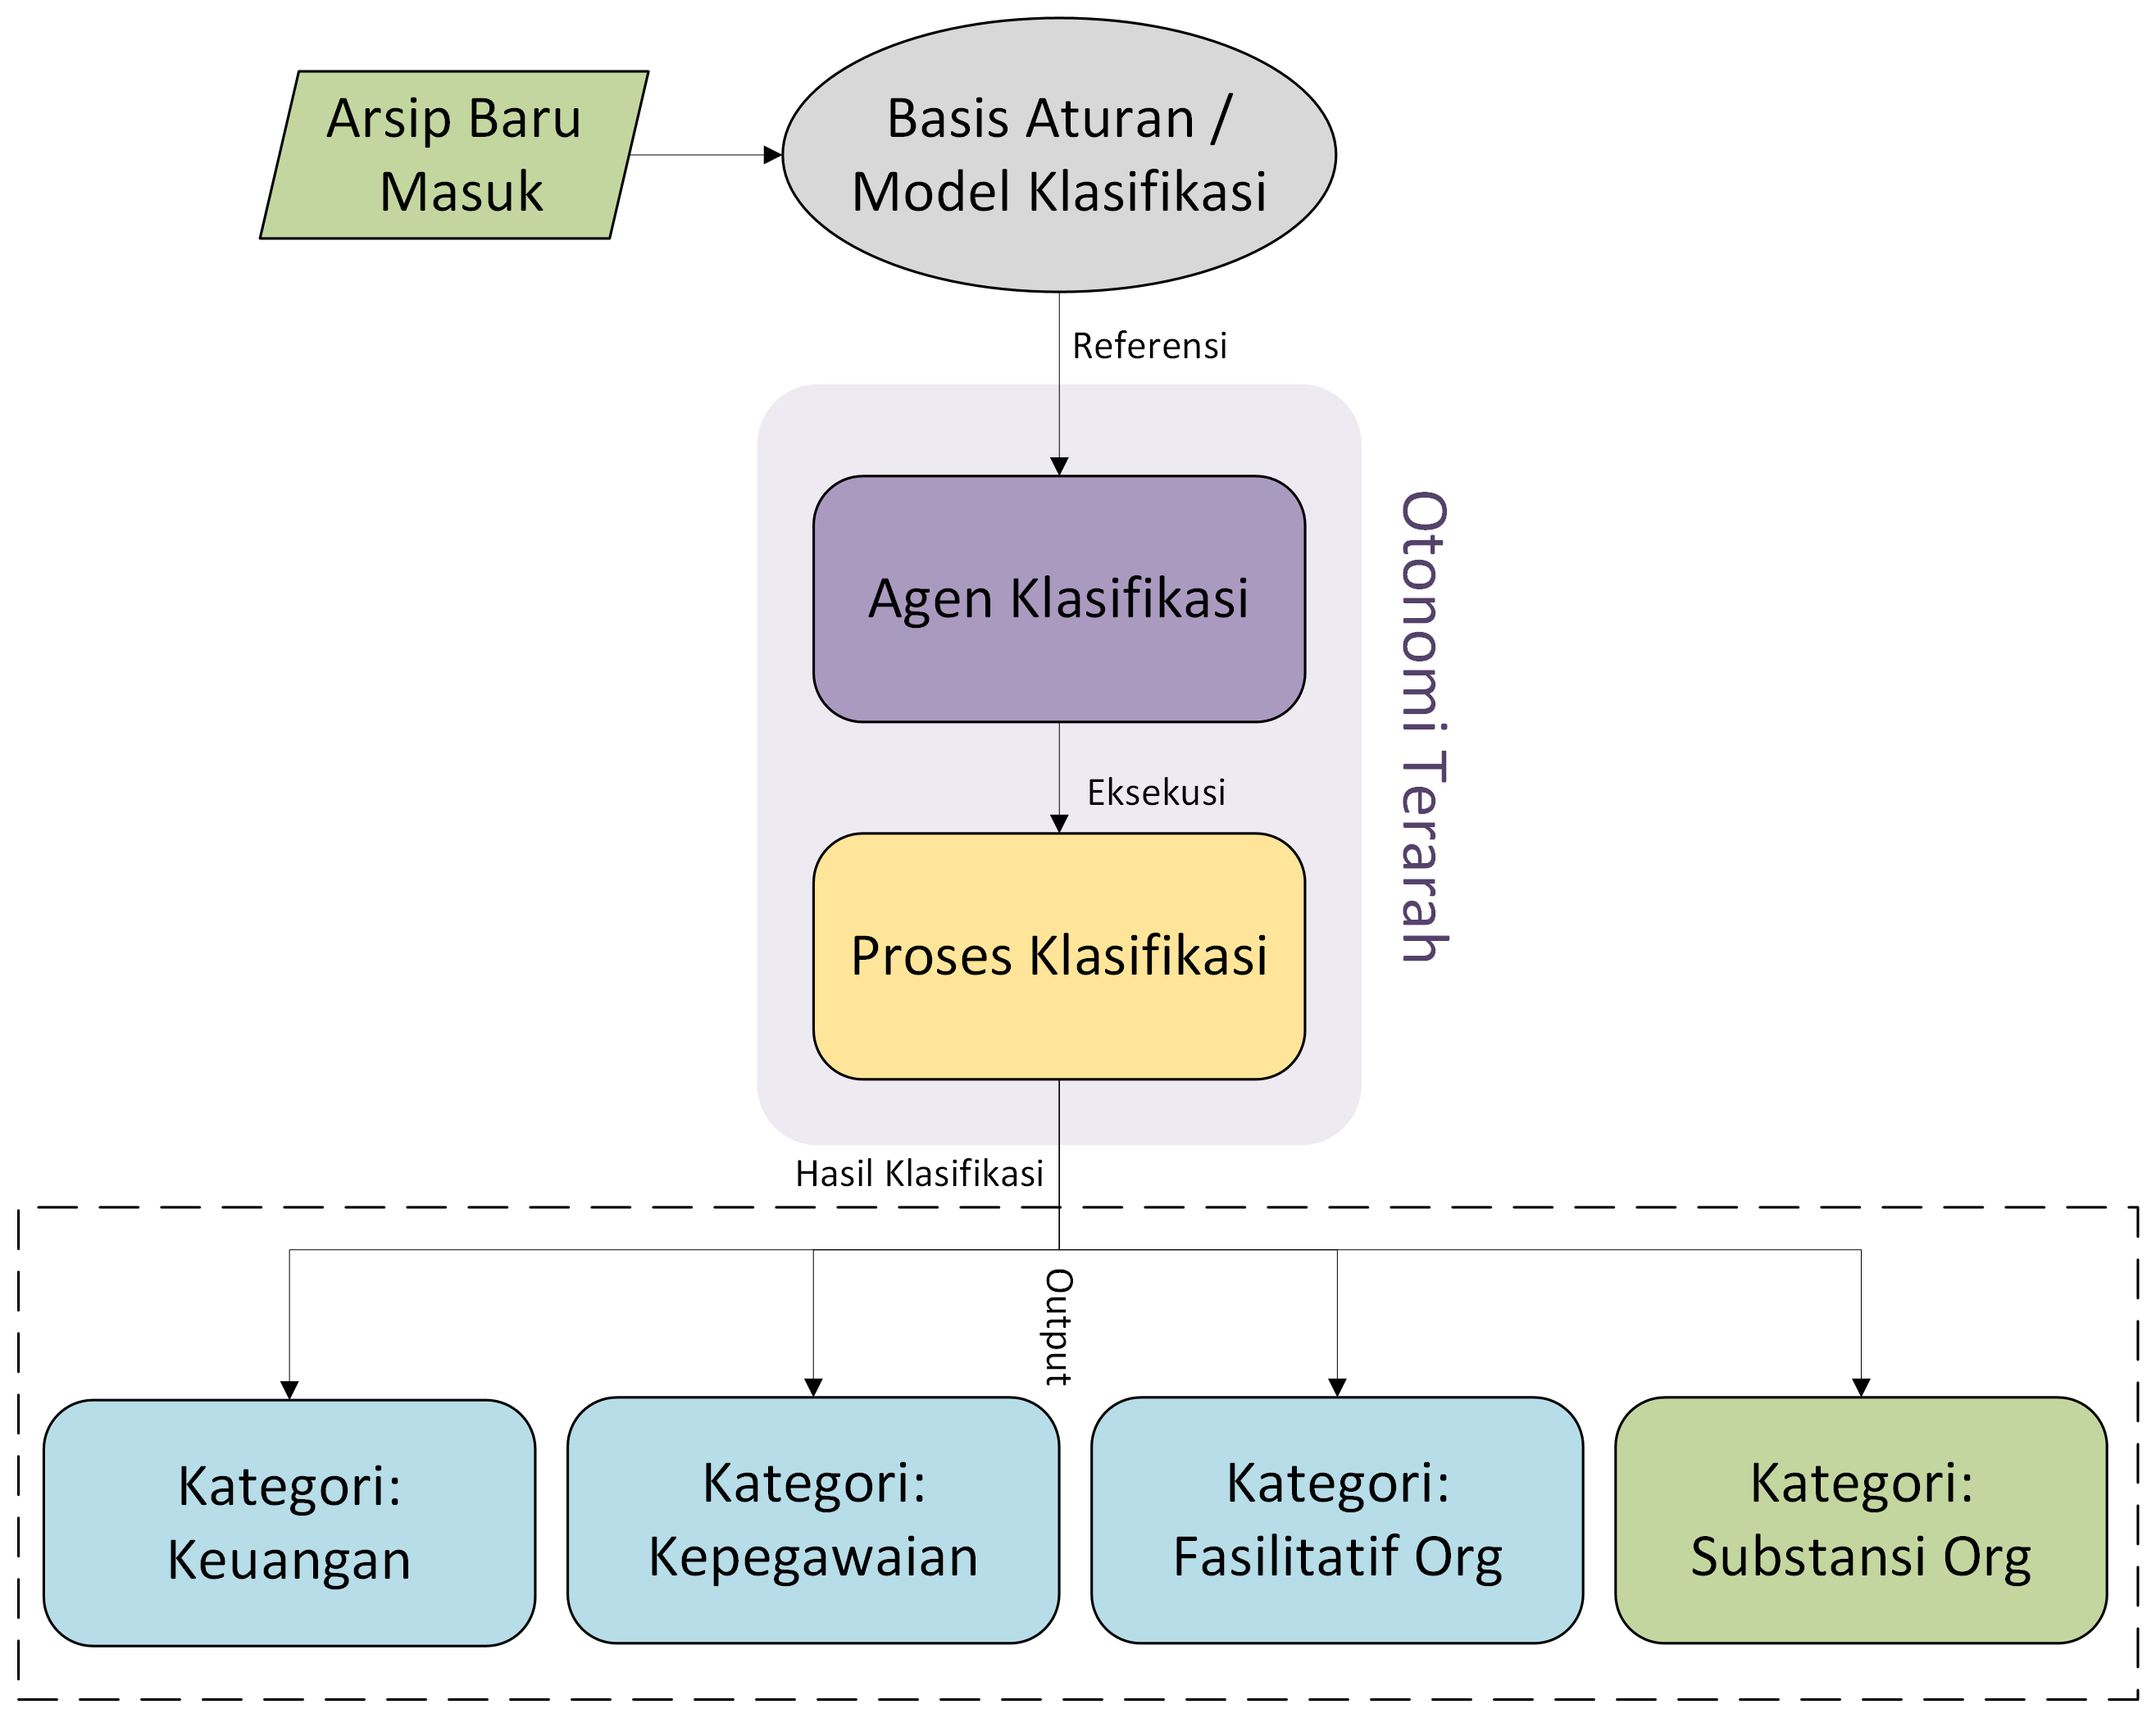
\includegraphics[width=0.6\linewidth]{media/media/image1.png}
\caption{Contoh Agen Otonom Menerapkan Aturan Klasifikasi}
\label{fig:agen_otonom}
\end{figure}

Relevansi untuk tata kelola kearsipan: (1) Konsistensi Proses: Dengan otonomi terarah, agen AI dapat secara konsisten menerapkan kebijakan dan prosedur kearsipan yang sama pada setiap arsip atau transaksi data, mengurangi variabilitas yang sering muncul akibat interpretasi manusia yang berbeda atau kelelahan. Misalnya, agen dapat secara otonom menerapkan aturan penamaan file standar atau mengalokasikan arsip ke folder yang tepat berdasarkan aturan klasifikasi. (2) Kemampuan untuk bekerja secara otonom memungkinkan penanganan volume data kearsipan yang besar secara efisien, tugas yang seringkali membebani sumber daya manusia.

\subsubsection{Proaktivitas Berbasis Aturan dan Tujuan}

Deskripsi Kapabilitas: Berbeda dengan sistem yang hanya reaktif, Agentic AI dapat mengambil inisiatif untuk bertindak guna mencapai tujuannya atau berdasarkan aturan yang telah diprogram. Agen tidak hanya menunggu perintah, tetapi dapat memicu tindakan berdasarkan kondisi tertentu atau untuk mencegah masalah potensial.

\begin{figure}[htbp]
\centering
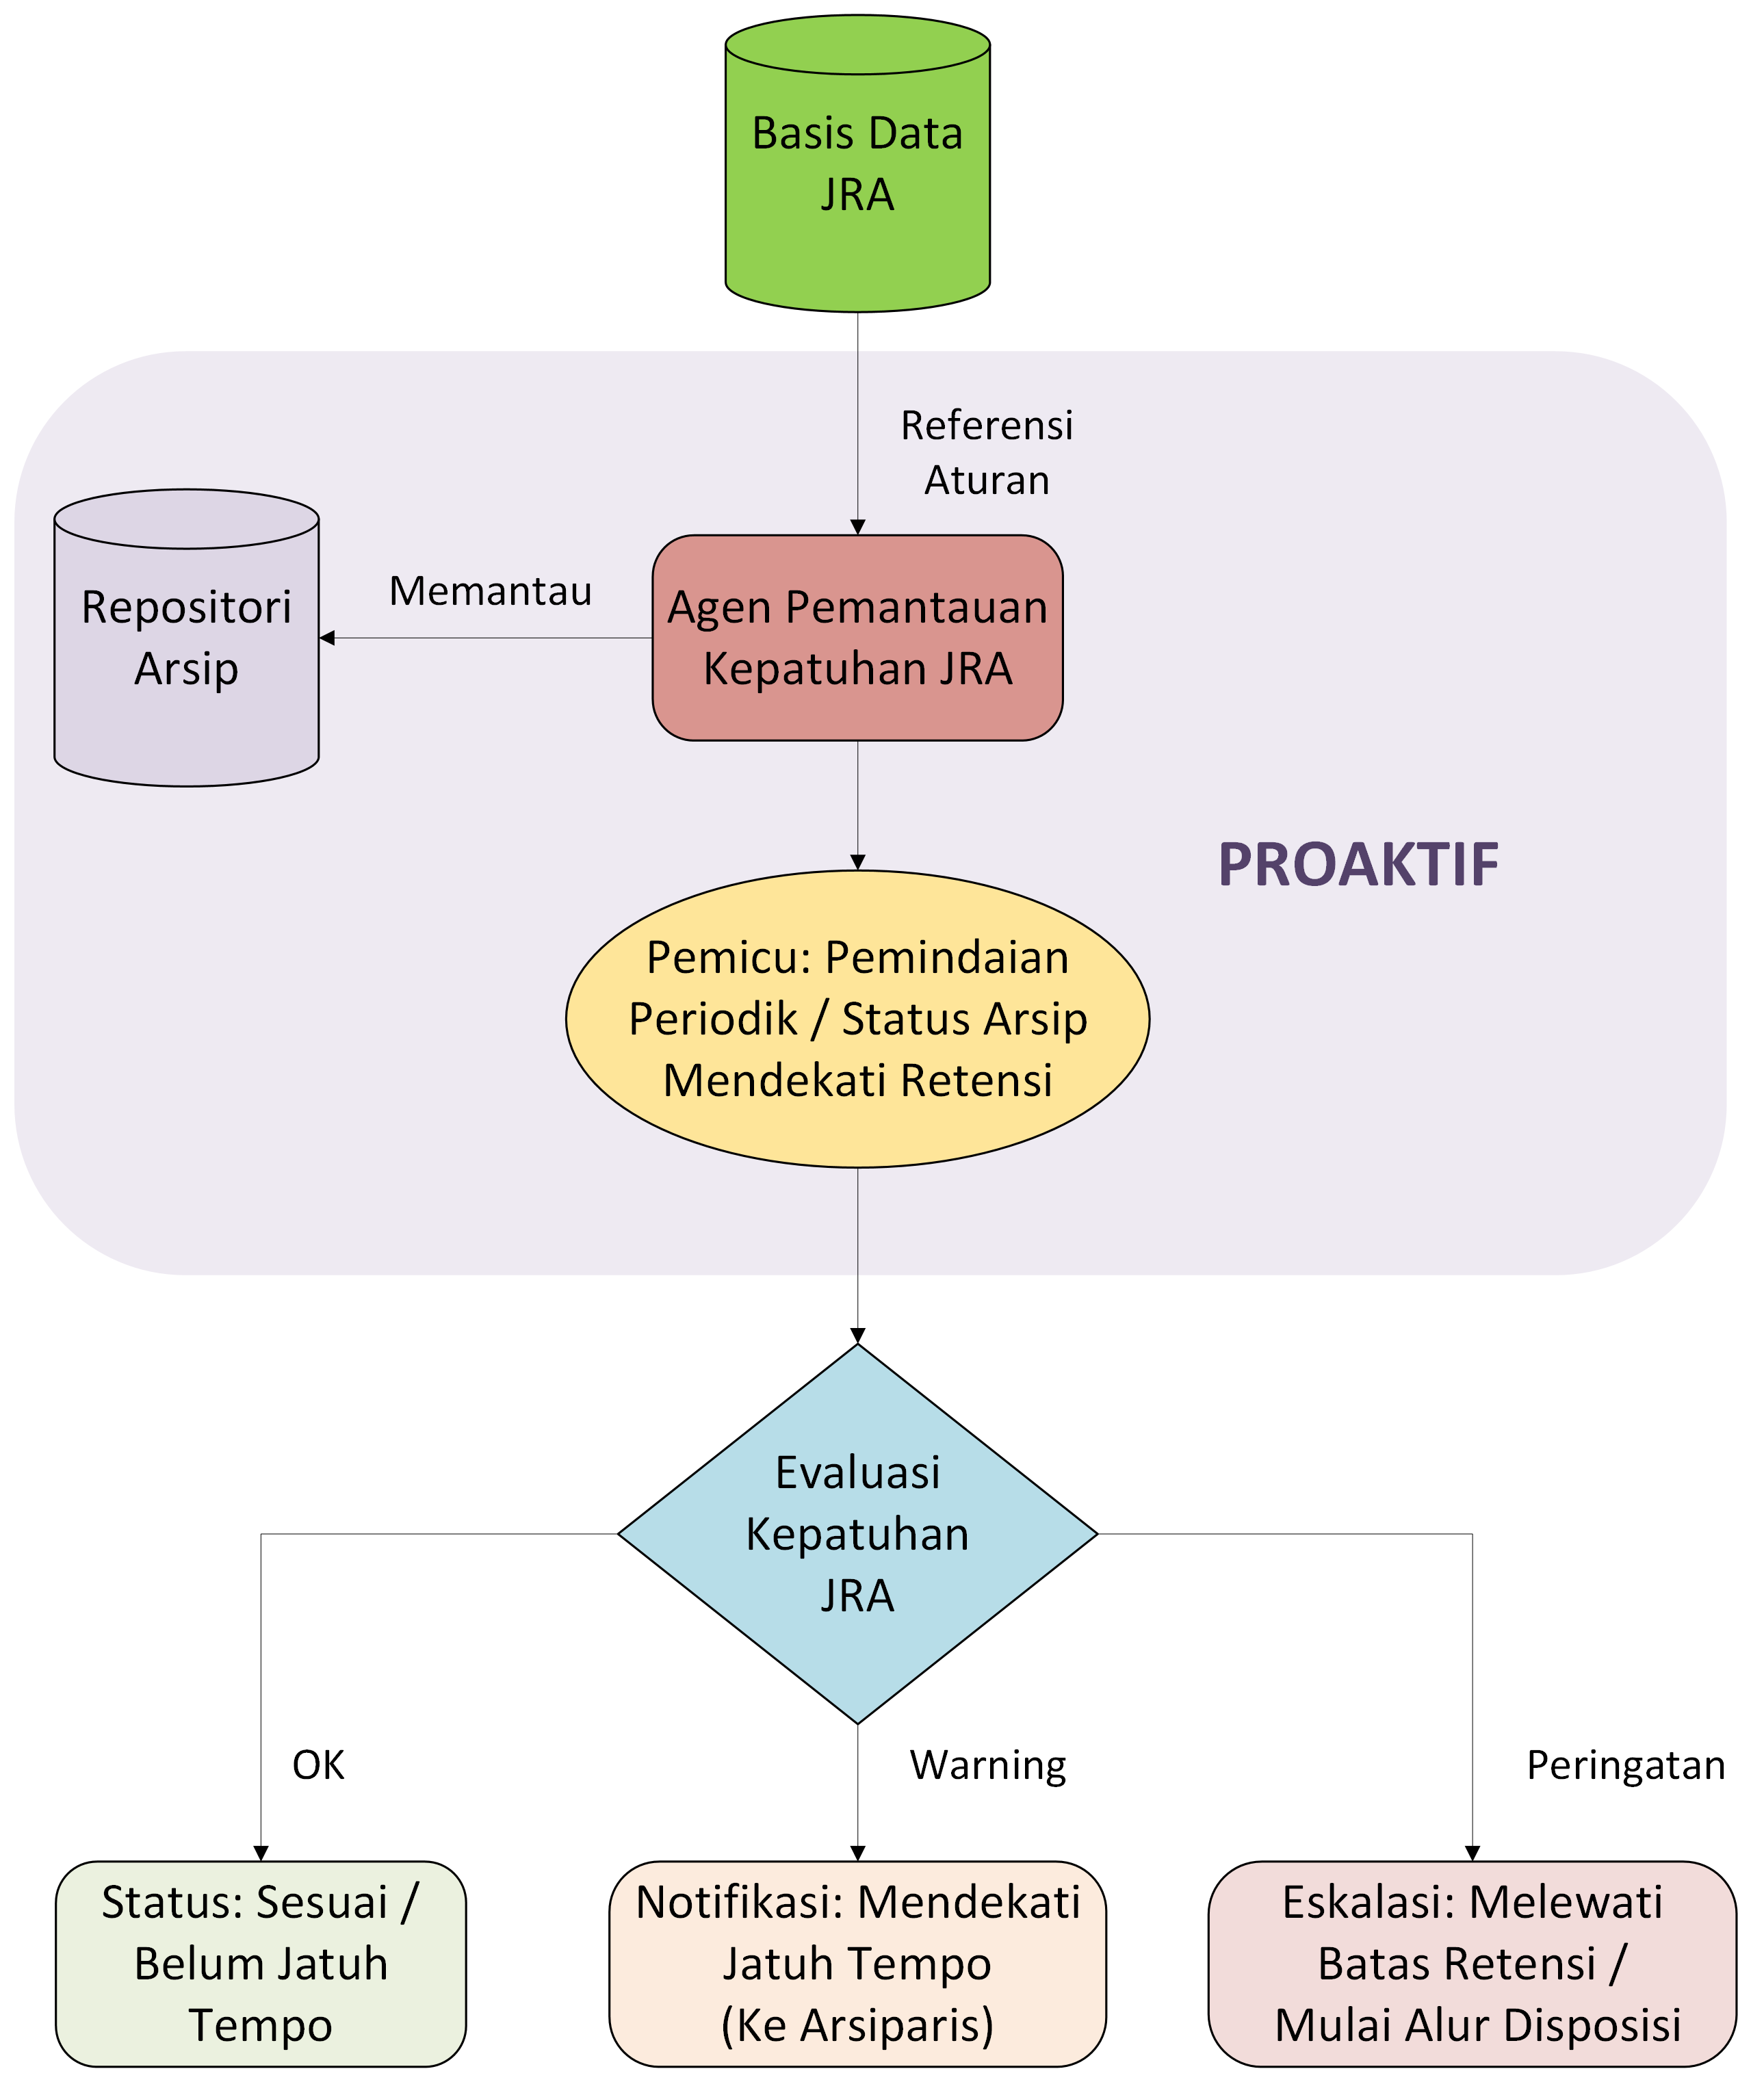
\includegraphics[width=0.6\linewidth]{media/media/image2.png}
\caption{Agen Proaktif Memantau Kepatuhan Standar Metadata}
\label{fig:agen_proaktif}
\end{figure}

Relevansi untuk tata kelola kearsipan: (1) Pemantauan Kepatuhan Aktif: Agen AI dapat secara proaktif memantau kepatuhan terhadap jadwal retensi arsip, kebijakan keamanan, atau standar metadata. Jika terdeteksi potensi pelanggaran atau ketidaksesuaian (misalnya, metadata yang hilang setelah periode waktu tertentu), agen dapat secara otomatis memberikan notifikasi, memulai alur kerja perbaikan, atau bahkan melakukan tindakan korektif sederhana. (2) Identifikasi Risiko Dini: Agen dapat dilatih untuk mengenali pola yang mengindikasikan risiko terhadap integritas atau keamanan arsip, dan secara proaktif mengambil langkah mitigasi atau memberi tahu penanggung jawab.(3) Pemeliharaan Struktur Data: Agen dapat proaktif memeriksa dan memperbaiki inkonsistensi dalam struktur metadata atau skema klasifikasi secara berkala.

\subsubsection{Kemampuan Belajar dan Adaptasi}

Deskripsi Kapabilitas: Agentic AI (terutama yang memanfaatkan machine learning) memiliki kemampuan untuk belajar dari data baru, interaksi, dan umpan balik (feedback) untuk meningkatkan kinerjanya seiring waktu. Agen dapat beradaptasi dengan perubahan pola data atau kebutuhan pengguna.

Relevansi untuk tata kelola kearsipan: (1) Peningkatan Akurasi Klasifikasi dan Ekstraksi Metadata: Melalui mekanisme Human-in-the-Loop (HITL), agen AI dapat belajar dari koreksi yang dilakukan oleh arsiparis, sehingga saran klasifikasi atau ekstraksi metadata otomatis menjadi semakin akurat. (2) Adaptasi terhadap Perubahan Kebijakan: Meskipun memerlukan konfigurasi ulang, agen yang adaptif dapat lebih mudah disesuaikan untuk mengikuti perubahan dalam kebijakan kearsipan atau standar metadata daripada melakukan perubahan manual pada seluruh sistem. (3) Optimasi Proses: Agen dapat belajar mengidentifikasi bottleneck atau inefisiensi dalam alur kerja kearsipan dan menyarankan atau mengimplementasikan optimasi.

\begin{figure}[htbp]
\centering
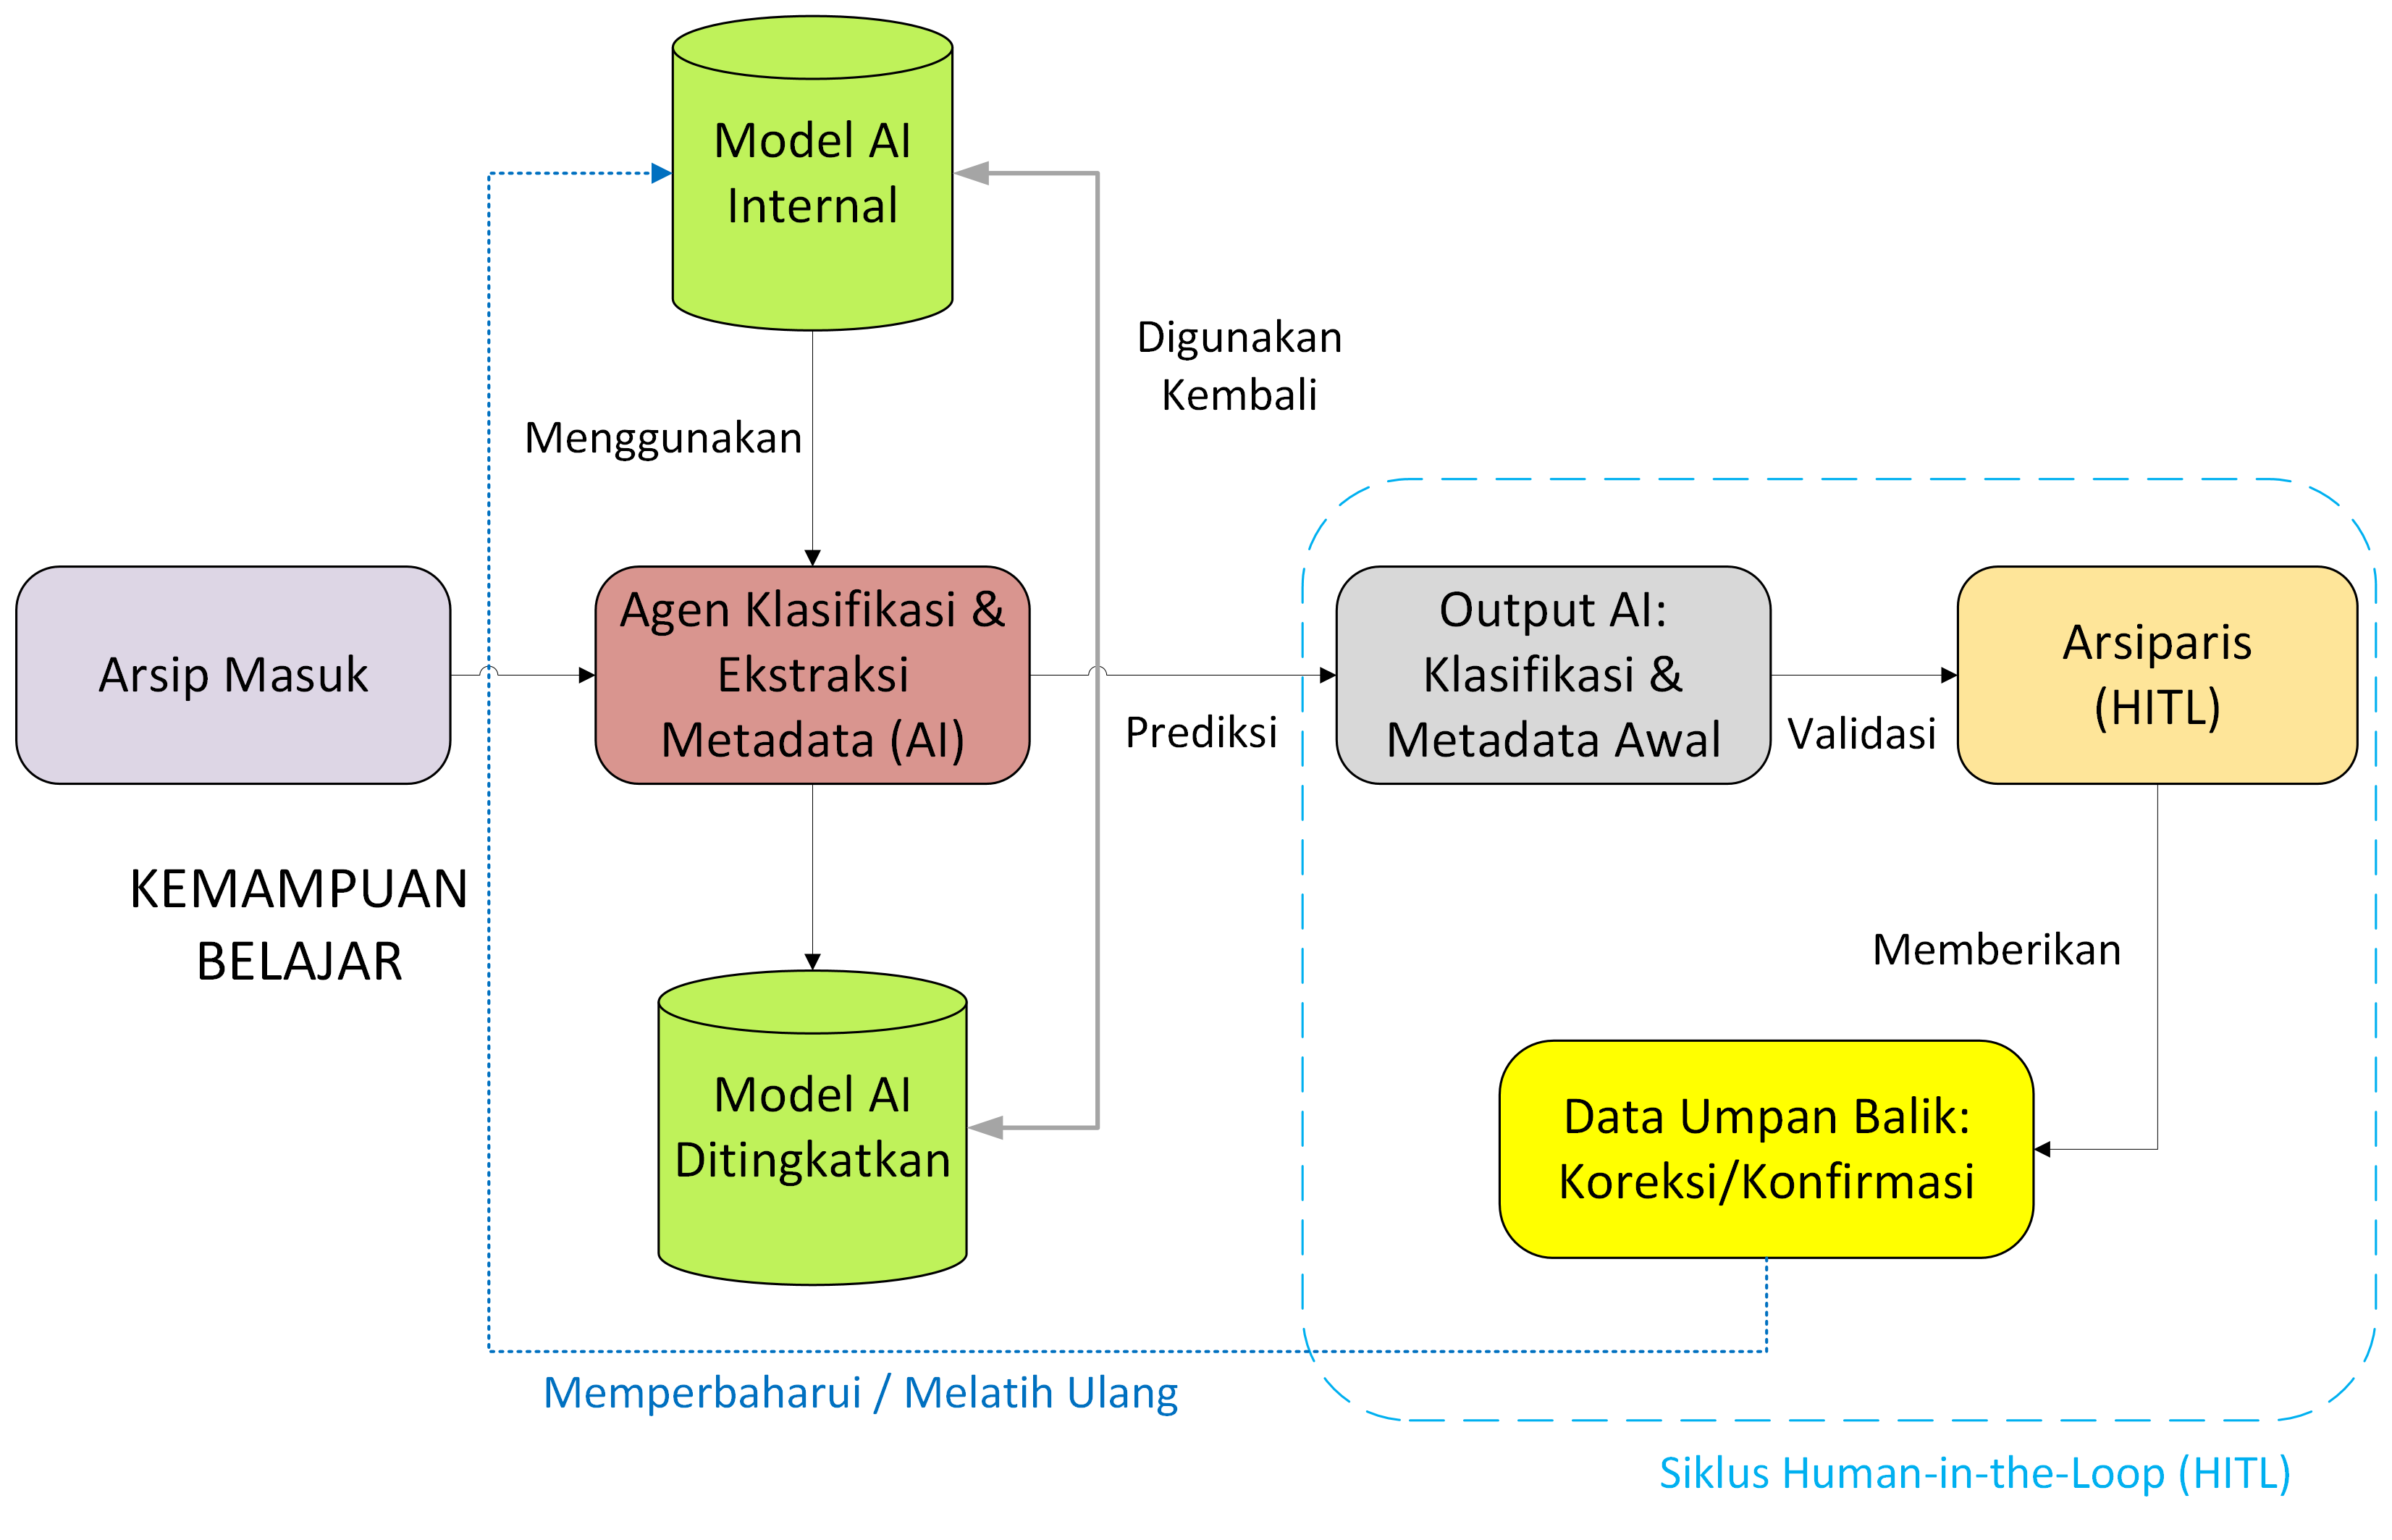
\includegraphics[width=0.6\linewidth]{media/media/image3.png}
\caption{Agen Pembelajar dengan Mekanisme HITL untuk Meningkatkan Akurasi Klasifikasi dan Ekstraksi Metadata}
\label{fig:agen_hitl}
\end{figure}

\subsubsection{Koordinasi dan Kolaborasi dalam Sistem Multi-Agen}

Deskripsi Kapabilitas: Agentic AI diimplementasikan dalam arsitektur Multi-Agent System (MAS), di mana berbagai agen dengan spesialisasi berbeda bekerja sama untuk mencapai tujuan yang lebih besar. Agen dapat berkomunikasi, bernegosiasi, dan mengoordinasikan tindakan. Relevansi untuk tata kelola kearsipan: (1) Pembagian Kerja yang Efisien: Tugas-tugas kompleks dalam tata kelola kearsipan (misalnya, mulai dari akuisisi hingga disposisi) dapat dipecah dan didelegasikan ke agen-agen spesialis (misalnya, Agen Akuisisi, Agen Metadata, Agen Retensi, Agen Layanan). (2) Alur Kerja Terotomatisasi dan Terintegrasi: Agen-agen dapat saling memicu tindakan secara berurutan atau paralel, menciptakan alur kerja tata kelola yang terotomatisasi. Contohnya, setelah Agen Akuisisi mendaftarkan arsip baru, Agen dapat memberi sinyal kepada Agen Metadata untuk memulai proses ekstraksi dan validasi metadata. (3) Peningkatan Konsistensi Lintas Fungsi: Dengan agen-agen yang beroperasi berdasarkan aturan dan tujuan bersama dalam MAS, konsistensi dapat dijaga tidak hanya dalam satu tugas, tetapi juga lintas berbagai fungsi tata kelola kearsipan.

\begin{figure}[htbp]
\centering
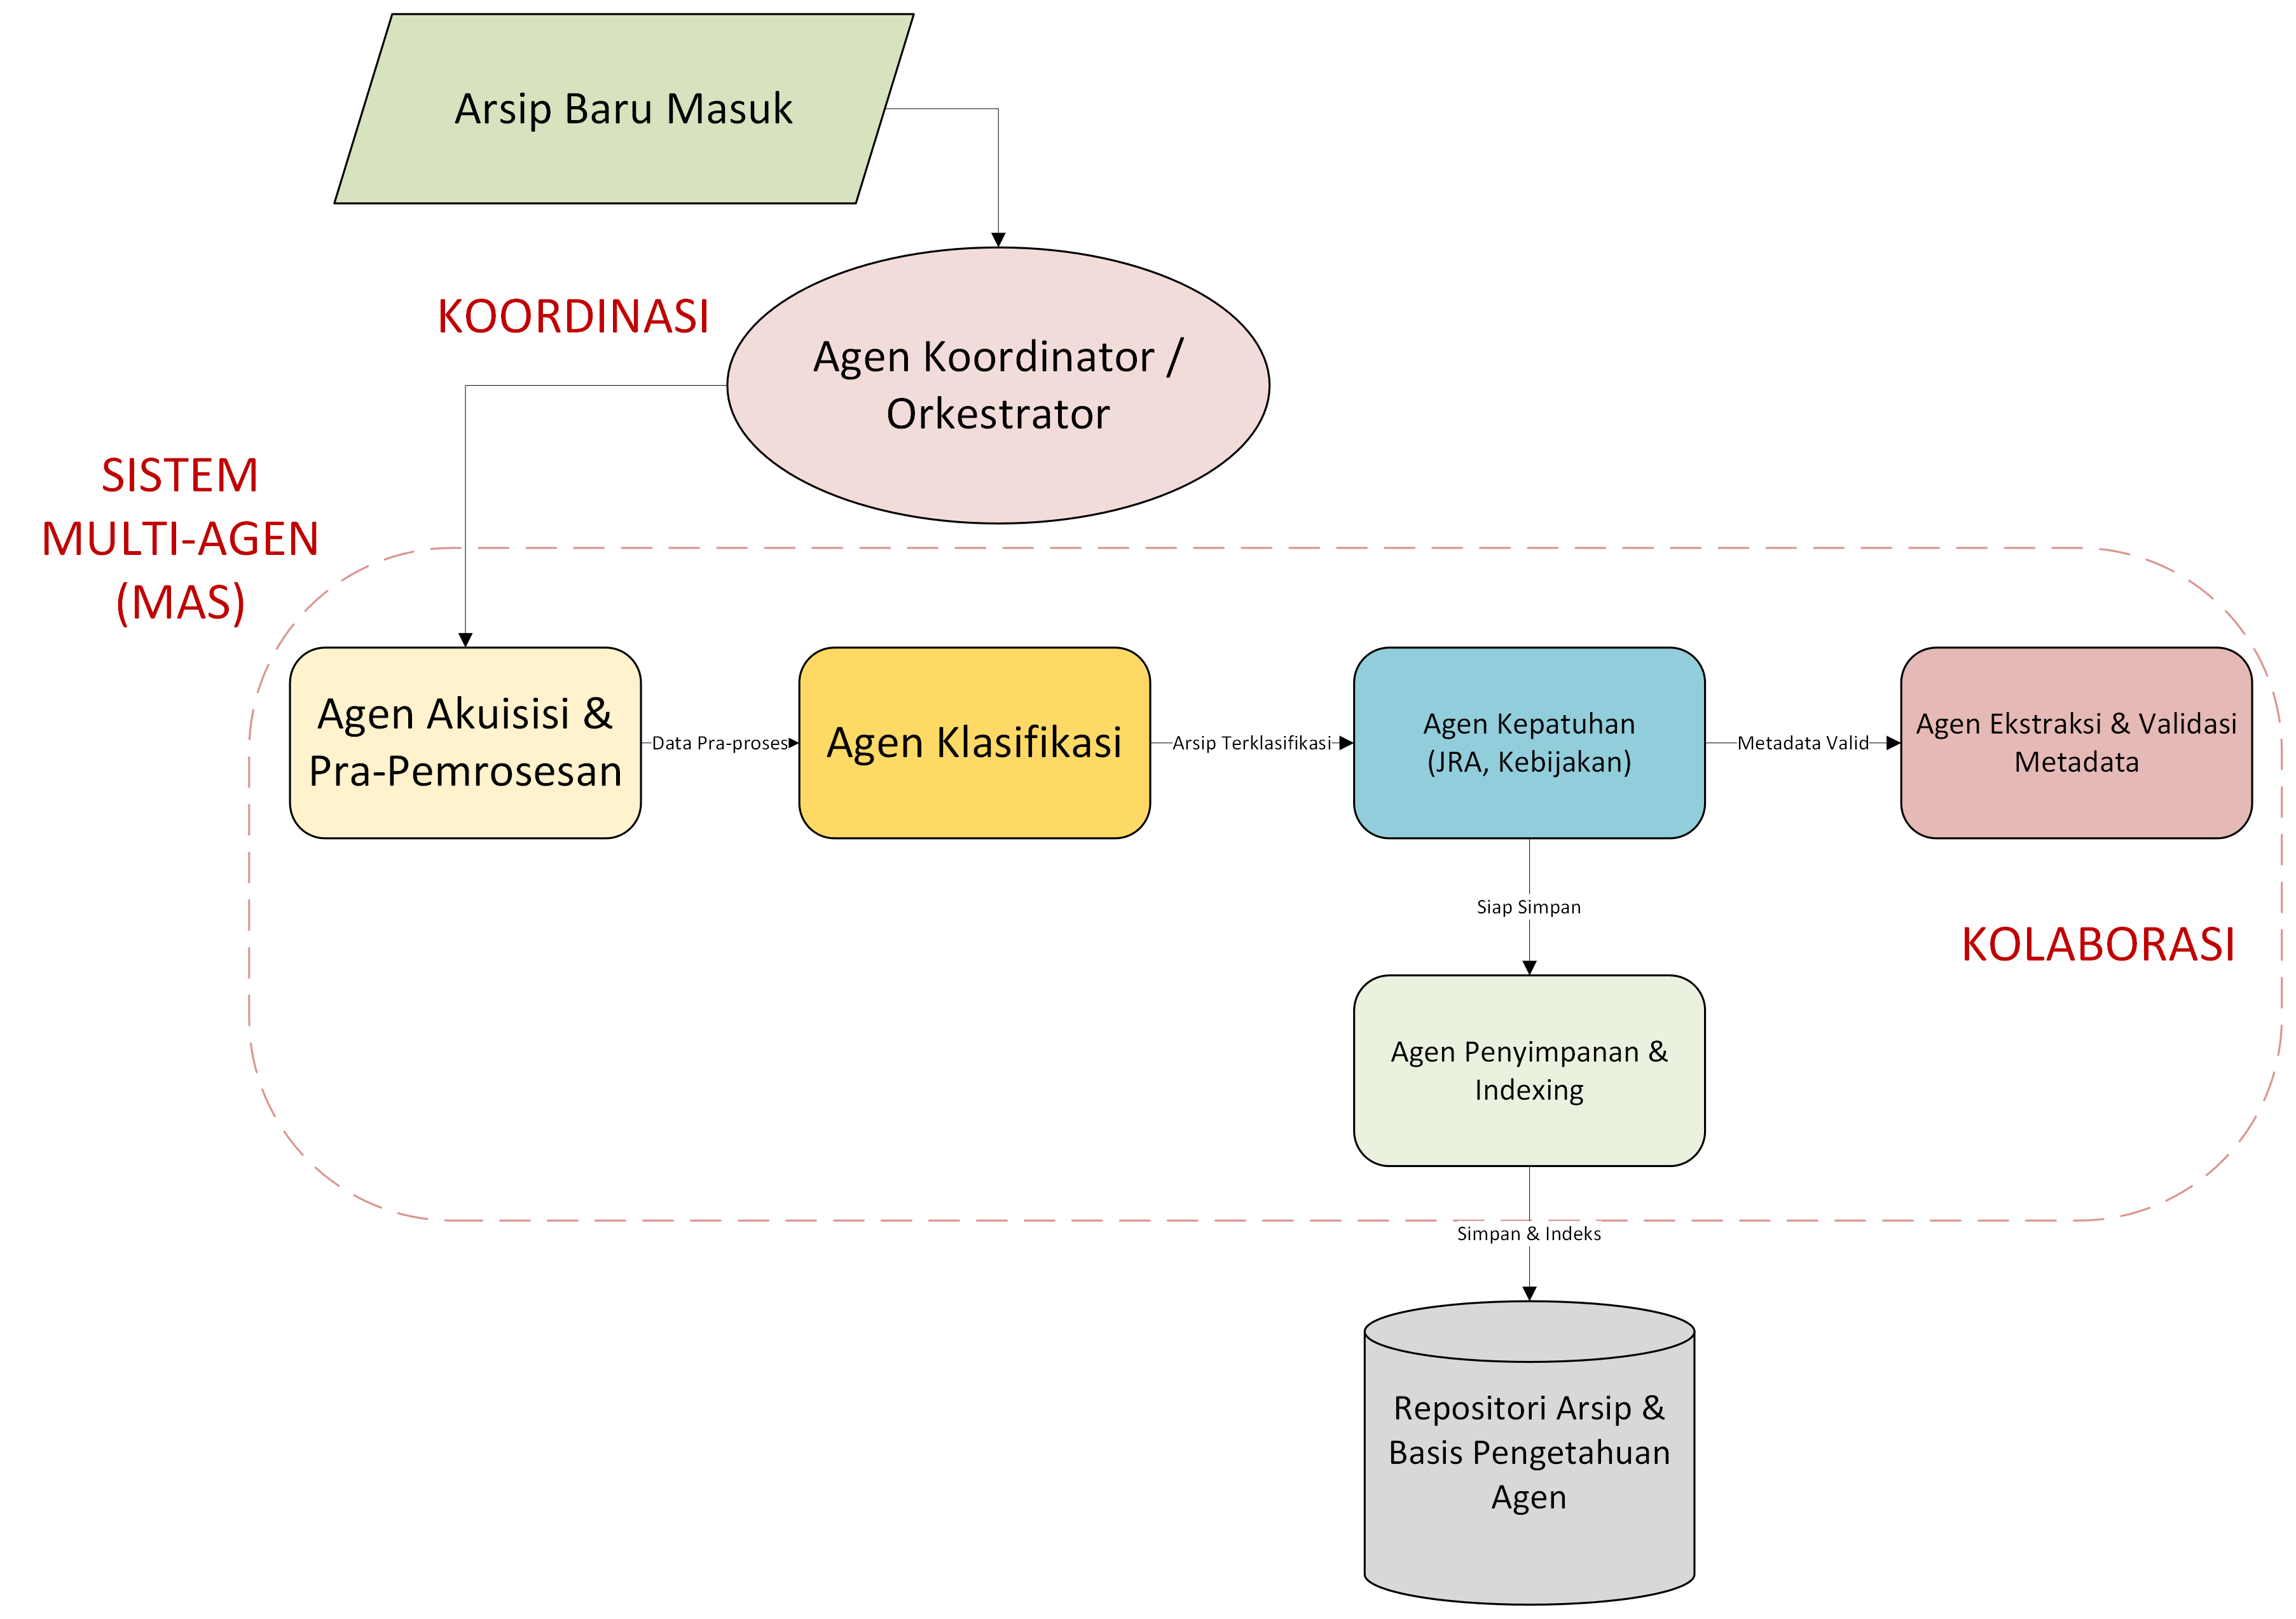
\includegraphics[width=0.7\linewidth]{media/media/image4.png}
\caption{Sistem Multi-Agen dalam Tata Kelola Data Kearsipan}
\label{fig:sistem_mas}
\end{figure}

\subsection{Kontribusi Agentic AI terhadap Indikator Kinerja Utama (IKU)}

Implementasi arsitektur Sistem Multi-Agen (MAS) berbasis Agentic AI sebagaimana diusulkan dalam penelitian ini diproyeksikan memberikan kontribusi signifikan dan positif terhadap pencapaian berbagai IKU yang menjadi tolak ukur keberhasilan tata kelola kearsipan. Dengan kemampuan otomatisasi cerdas, peningkatan konsistensi, dan pemrosesan data yang lebih akurat, sistem ini berpotensi meningkatkan skor IKU di berbagai aspek fundamental.

\begin{figure}[htbp]
\centering
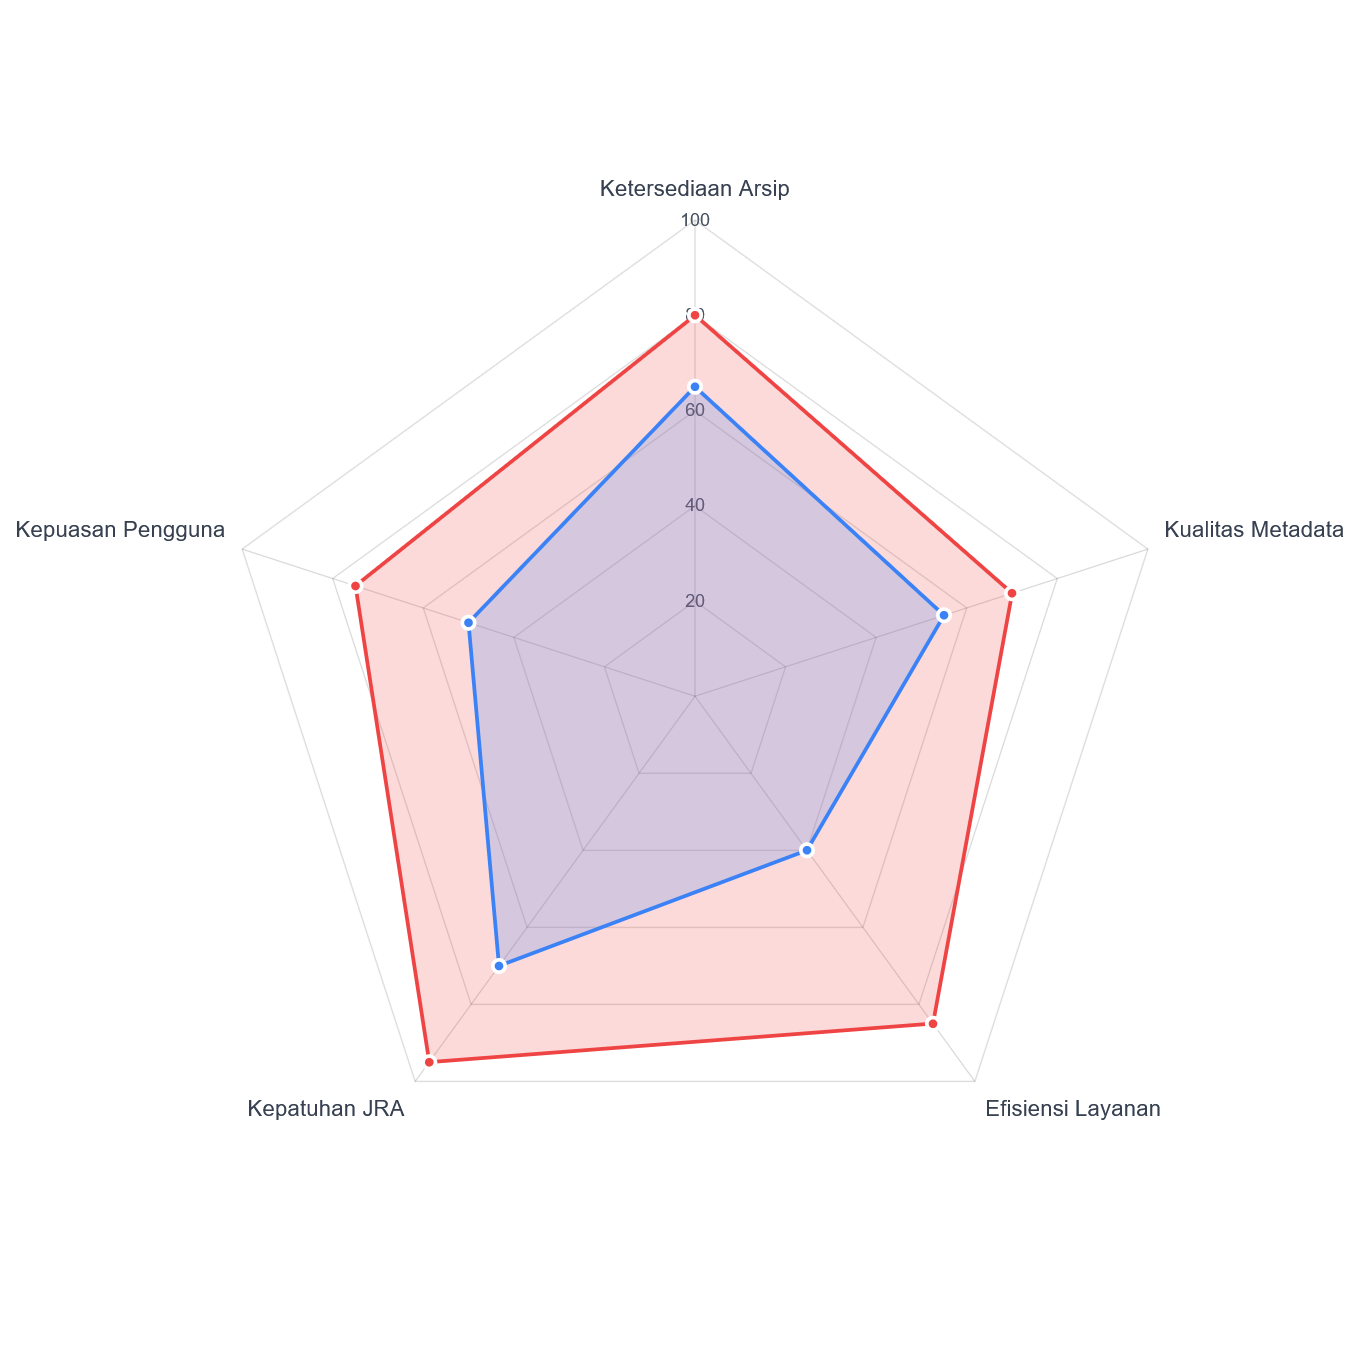
\includegraphics[width=0.6\linewidth]{media/media/image5.png}
\caption{Proyeksi Peningkatan Skor IKU dari Pemanfaatan \emph{Agentic AI}}
\label{fig:proyeksi_iku}
\end{figure}

Terdapat lima IKU yang menjadi target penerapan Agentic AI tata kelola data ini, yaitu: (a) Ketersediaan dan Aksesibilitas Arsip, (b) Kualitas metadata dan struktur informasi, Efisiensi Layanan informasi kearsipan. (c) kepatuhan terhadap regulasi dan kebijakan, serta Efisiensi Operasional dan Tata Kelola Secara Umum

\subsubsection{IKU Ketersediaan dan Aksesibilitas Arsip}

IKU yang relevan berfokus pada dua area utama yaitu efisiensi pengolahan dan kecepatan akses arsip. Untuk IKU terkait pengolahan seperti mengurangi backlog dan melengkapi deskripsi arsip, diperlukan Agentic AI yang mampu mengotomatisasi proses akuisisi, klasifikasi, dan ekstraksi metadata. Sementara itu, untuk IKU terkait akses seperti mempercepat waktu temu kembali informasi, dibutuhkan agen AI yang unggul dalam indexing cerdas dan layanan pencarian instan.

\begin{table}[htbp]
\centering
\caption{Proyeksi Kontribusi \emph{Agentic AI} terhadap IKU Ketersediaan dan Aksesibilitas Arsip}
\label{tab:iku_ketersediaan}
\begin{tabular}{|p{0.3\linewidth}|p{0.65\linewidth}|}
\hline
\textbf{IKU} & \textbf{Kontribusi Agentic AI} \\
\hline
\multicolumn{2}{|c|}{\emph{(Tabel detail tersedia dalam dokumen asli)}} \\
\hline
\end{tabular}
\end{table}

\subsubsection{IKU Kualitas Metadata dan Struktur Informasi}

IKU yang relevan secara spesifik menargetkan berbagai aspek peningkatan kualitas metadata, mulai dari kelengkapan, akurasi, konsistensi penggunaan skema, hingga pemenuhan standar interoperabilitas.

Untuk mencapai hal ini, hubungan dengan Agentic AI sangatlah krusial, di mana peran utama dipegang oleh Agen Ekstraksi \& Validasi Metadata untuk mengotomatiskan pengisian dan pemeriksaan data. Kinerjanya kemudian disempurnakan oleh Agen Pembelajar (HITL) yang terus meningkatkan akurasi, serta agen lain yang menjamin penggunaan skema dan standar secara konsisten.

\begin{table}[htbp]
\centering
\caption{Proyeksi Kontribusi \emph{Agentic AI} terhadap IKU Kualitas Metadata dan Struktur Informasi}
\label{tab:iku_metadata}
\begin{tabular}{|p{0.3\linewidth}|p{0.65\linewidth}|}
\hline
\textbf{IKU} & \textbf{Kontribusi Agentic AI} \\
\hline
\multicolumn{2}{|c|}{\emph{(Tabel detail tersedia dalam dokumen asli)}} \\
\hline
\end{tabular}
\end{table}

\subsubsection{IKU Efisiensi Layanan Informasi Kearsipan}

IKU yang relevan berpusat pada peningkatan kualitas layanan pengguna, yang diukur dari kecepatan respons, tingkat kepuasan, hingga kemampuan pengguna untuk melakukan layanan mandiri (self-service). Untuk memenuhi target ini, hubungan dengan Agentic AI sangatlah vital, dengan Agen Layanan Cerdas sebagai komponen utama yang berfungsi sebagai garda terdepan untuk interaksi pengguna, seperti menangani pencarian bahasa alami (NLP) dan otomasi respons. Keberhasilan agen ini didukung oleh agen di belakang layar yang memastikan metadata berkualitas dan indexing yang optimal, sehingga informasi yang disajikan selalu relevan dan akurat.

\begin{table}[htbp]
\centering
\caption{Proyeksi Kontribusi \emph{Agentic AI} terhadap IKU Efisiensi Layanan Informasi Kearsipan}
\label{tab:iku_layanan}
\begin{tabular}{|p{0.3\linewidth}|p{0.65\linewidth}|}
\hline
\textbf{IKU} & \textbf{Kontribusi Agentic AI} \\
\hline
\multicolumn{2}{|c|}{\emph{(Tabel detail tersedia dalam dokumen asli)}} \\
\hline
\end{tabular}
\end{table}

\subsubsection{IKU Kepatuhan terhadap Regulasi dan Kebijakan}

IKU yang relevan berfokus pada penegakan kepatuhan dan keamanan, mencakup ketaatan pada kebijakan, Jadwal Retensi Arsip (JRA), hingga klasifikasi keamanan dan hak akses yang tepat. Untuk mencapai IKU tersebut, peran sentral dipegang oleh Agen Kepatuhan yang secara proaktif memantau kebijakan, mengelola siklus hidup arsip sesuai JRA, dan menyediakan audit trail untuk mempermudah audit. Aspek keamanan dan respons insiden kemudian diperkuat oleh agen spesialis yang mampu mengotomatisasi klasifikasi keamanan serta mendeteksi potensi pelanggaran secara real-time, mengubah manajemen risiko dari reaktif menjadi lebih preventif.

\subsubsection{IKU Terkait Efisiensi Operasional dan Tata Kelola Secara Umum}

IKU yang relevan mengukur dampak strategis dari sistem Agentic AI pada tingkat institusional, yang terhubung langsung dengan target efisiensi, biaya, dan program pemerintah seperti Reformasi Birokrasi, SPBE, dan SAKIP. Hubungannya bersifat holistik: IKU ini dipenuhi melalui efisiensi kolektif dari semua Agen Operasional yang mengotomatisasi tugas rutin untuk menekan biaya dan waktu, serta membebaskan SDM untuk pekerjaan strategis. Keberhasilan ini kemudian diorkestrasi oleh Agen Koordinator untuk alur kerja yang optimal, dan dibuktikan melalui data terukur dari Agen Analitik \& Pelaporan untuk mendukung akuntabilitas kinerja.

Dengan demikian, implementasi Agentic AI tidak hanya diproyeksikan sebagai solusi teknis untuk tugas-tugas spesifik, tetapi sebagai sebuah pendekatan strategis yang berpotensi secara holistik meningkatkan kinerja kearsipan. Kemampuan sistem untuk bekerja secara konsisten, proaktif, dan adaptif, akan menjadi pendorong utama dalam mencapai target-target IKU yang lebih optimal, sekaligus memperkuat peran fungsi kearsipan dalam mendukung tujuan organisasi yang lebih luas. Penting untuk dicatat bahwa realisasi penuh dari proyeksi kontribusi ini akan bergantung pada kualitas desain sistem, integrasi yang tepat dengan proses bisnis yang ada, serta dukungan organisasional yang memadai.

\subsection{Model Konseptual Pemanfaatan Agentic AI dalam Tata Kelola Kearsipan}

Berdasarkan analisis kapabilitas Agentic AI dan kebutuhan mendasar akan konsistensi serta struktur dalam tata kelola data kearsipan, penelitian ini mengusulkan sebuah model konseptual arsitektur Sistem Multi-Agen (MAS). Model ini dirancang untuk merepresentasikan dan mengotomatisasi berbagai fungsi kunci dalam siklus hidup arsip dan proses tata kelola, dengan tujuan utama meningkatkan kualitas, efisiensi, dan kepatuhan. Arsitektur pada Gambar 6 terdiri dari beberapa komponen agen utama yang berinteraksi secara terkoordinasi.

\subsubsection{Agen Koordinator/Orchestrator}

Bertindak sebagai pusat pengendali dan pengatur alur kerja dalam MAS. Agen ini menerima input awal (misalnya, arsip baru yang masuk), mendelegasikan tugas ke agen-agen spesialis yang sesuai, memantau progres pelaksanaan tugas, dan mengelola komunikasi antar agen jika diperlukan.

Fungsi Kunci -- (a). Manajemen antrian tugas dan prioritisasi. Delegasi tugas berdasarkan spesialisasi agen dan kondisi sistem. (b). Resolusi konflik sumber daya atau prioritas antar agen. (c). Mengumpulkan status dan laporan parsial dari agen spesialis. Agen ini berkontribusi dalam memastikan bahwa setiap arsip melewati tahapan tata kelola yang benar secara berurutan atau paralel sesuai definisi alur kerja, sehingga mengurangi variasi proses.

\subsubsection{Agen Akuisisi \& Pra-pemrosesan}

Bertanggung jawab untuk mendeteksi, menerima, dan melakukan persiapan awal terhadap arsip yang baru masuk ke dalam sistem.

Fungsi Kunci -- (a). Identifikasi otomatis arsip baru dari berbagai sumber (misalnya, email, folder bersama, sistem lain). (2). Registrasi awal arsip (pemberian nomor identifikasi unik). (3). Ekstraksi metadata teknis dasar (misalnya, tipe file, ukuran, tanggal pembuatan). (3). Konversi format file ke standar yang ditetapkan, deteksi duplikasi awal. Agen ini berkontribusi dalam memastikan semua arsip baru tercatat secara seragam dan melalui tahap persiapan standar sebelum diproses lebih lanjut.

\subsubsection{Agen Klasifikasi}

Agen Klasifikasi berperan dalam menerapkan skema klasifikasi kearsipan yang telah ditetapkan pada setiap arsip.

Fungsi Kunci -- (a) Analisis konten arsip (menggunakan NLP atau teknik lain) dan/atau atribut metadata. (b) Penerapan aturan klasifikasi bisnis atau model pembelajaran mesin untuk menentukan kategori klasifikasi yang tepat. (c). Pemberian label klasifikasi keamanan jika diperlukan. (d) Menggunakan mekanisme HITL untuk kasus ambigu atau validasi klasifikasi sensitif. Agen ini berkontribusi dalam menjamin penerapan skema klasifikasi yang seragam di seluruh organisasi, yang krusial untuk organisasi arsip yang logis dan temu kembali yang efektif.

\subsubsection{Agen Ekstraksi \& Validasi Metadata}

Bertugas mengekstrak informasi deskriptif, administratif, dan teknis dari arsip serta memvalidasinya terhadap standar metadata yang berlaku.

Fungsi Kunci -- (a) Ekstraksi otomatis entitas (nama, tempat, tanggal, organisasi, subjek kunci) dari konten arsip. (b) Pengisian otomatis kolom metadata berdasarkan informasi yang diekstrak atau konteks lain. (c) Validasi kelengkapan metadata wajib, format data, dan kesesuaian dengan kamus istilah terkontrol (tesaurus). (d) Pemberian skor kualitas metadata. (e) Menandai metadata yang memerlukan perhatian atau koreksi manual (HITL). Agen ini berkontribusi secara signifikan meningkatkan kualitas, kelengkapan, dan standarisasi metadata, yang merupakan tulang punggung dari arsip yang terstruktur dan mudah diakses.

\subsubsection{Agen Kepatuhan}

Agen kepatuhan berperan dalam memantau dan memastikan kepatuhan arsip dan proses pengelolaannya terhadap regulasi eksternal dan kebijakan internal.

Fungsi Kunci -- (a) Pemantauan proaktif terhadap JRA, mengidentifikasi arsip yang mendekati atau melewati masa retensi. (b) Memulai alur kerja disposisi (pemusnahan atau transfer) dengan notifikasi dan permintaan persetujuan ke arsiparis. (c) Memantau kepatuhan terhadap kebijakan keamanan dan hak akses. (d) Menghasilkan audit trail untuk tindakan kepatuhan. Agen ini berkontribusi terhadap menegakkan penerapan aturan secara konsisten, mengurangi risiko hukum dan operasional, serta memastikan arsip dikelola sesuai siklus hidup yang ditetapkan.

\subsubsection{Agen Penyimpanan dan Indexing}

Agen ini bertanggung jawab untuk menyimpan arsip (fisik atau digital) dan metadatanya ke dalam repositori yang sesuai, serta memastikan arsip terindeks dengan baik untuk pencarian.

Fungsi Kunci -- (a) Penempatan arsip digital ke lokasi penyimpanan yang aman dan sesuai. (b) Pembuatan dan pembaruan indeks pencarian berdasarkan metadata dan konten. (c) Manajemen versi arsip. (d) Memantau integritas file digital. Agen ini berkontribusi memastikan arsip disimpan secara teratur dan dapat ditemukan dengan mudah melalui mekanisme pencarian yang efisien.

\subsubsection{Agen Layanan Informasi}

Agen ini berperan dalam menyediakan antarmuka bagi pengguna untuk mencari dan mengakses arsip.

Fungsi Kunci -\/- Memproses query pencarian (termasuk bahasa alami). (b) Menyajikan hasil pencarian yang relevan. (c) Mengelola permintaan akses dan menerapkan kontrol akses. (d) Menangani permintaan informasi rutin secara otomatis. Agen ini berkontribusi menyediakan titik akses yang konsisten dan terstruktur ke koleksi arsip.

\subsubsection{Agen Analitik dan Pelaporan IKU}

Agen ini berperan dalam mengumpulkan data kinerja dari berbagai agen operasional dan sistem, menghitung skor IKU, dan menyajikan laporan atau dashboard kinerja. Fungsi Kunci -- (a) Integrasi dengan log aktivitas agen dan metrik sistem. (b) Kalkulasi otomatis IKU berdasarkan formula yang telah ditetapkan. (c) Visualisasi data kinerja dan tren IKU. (d) Memberikan rekomendasi atau peringatan jika IKU di bawah target.

Agen ini berkontribusi dalam menyediakan mekanisme pengukuran yang objektif dan konsisten terhadap efektivitas tata kelola, mendukung siklus perbaikan berkelanjutan.

\subsubsection{Interaksi dan Alur Kerja Antar Agen}

Dalam model ini, interaksi dan alur kerja antar agen diatur untuk memastikan proses yang terkoordinasi dan efisien. Prosesnya diawali ketika sebuah arsip baru diterima oleh Agen Koordinator, yang bertindak sebagai pusat orkestrasi sistem. Dari sana, tugas didelegasikan ke Agen Akuisisi \& Pra-pemrosesan untuk penanganan awal. Setelah tahap ini selesai, arsip kemudian diteruskan secara berurutan ke Agen Klasifikasi untuk pengelompokan dan Agen Ekstraksi \& Validasi Metadata untuk pengayaan informasi. Secara bersamaan, Agen Kepatuhan dapat terus memantau status arsip untuk memastikan kesesuaian dengan kebijakan yang berlaku. Pada tahap akhir, setelah semua validasi dan klasifikasi selesai, Agen Penyimpanan \& Indexing akan menyimpan arsip secara aman dan mengindeksnya agar dapat ditemukan kembali.

\begin{figure}[htbp]
\centering
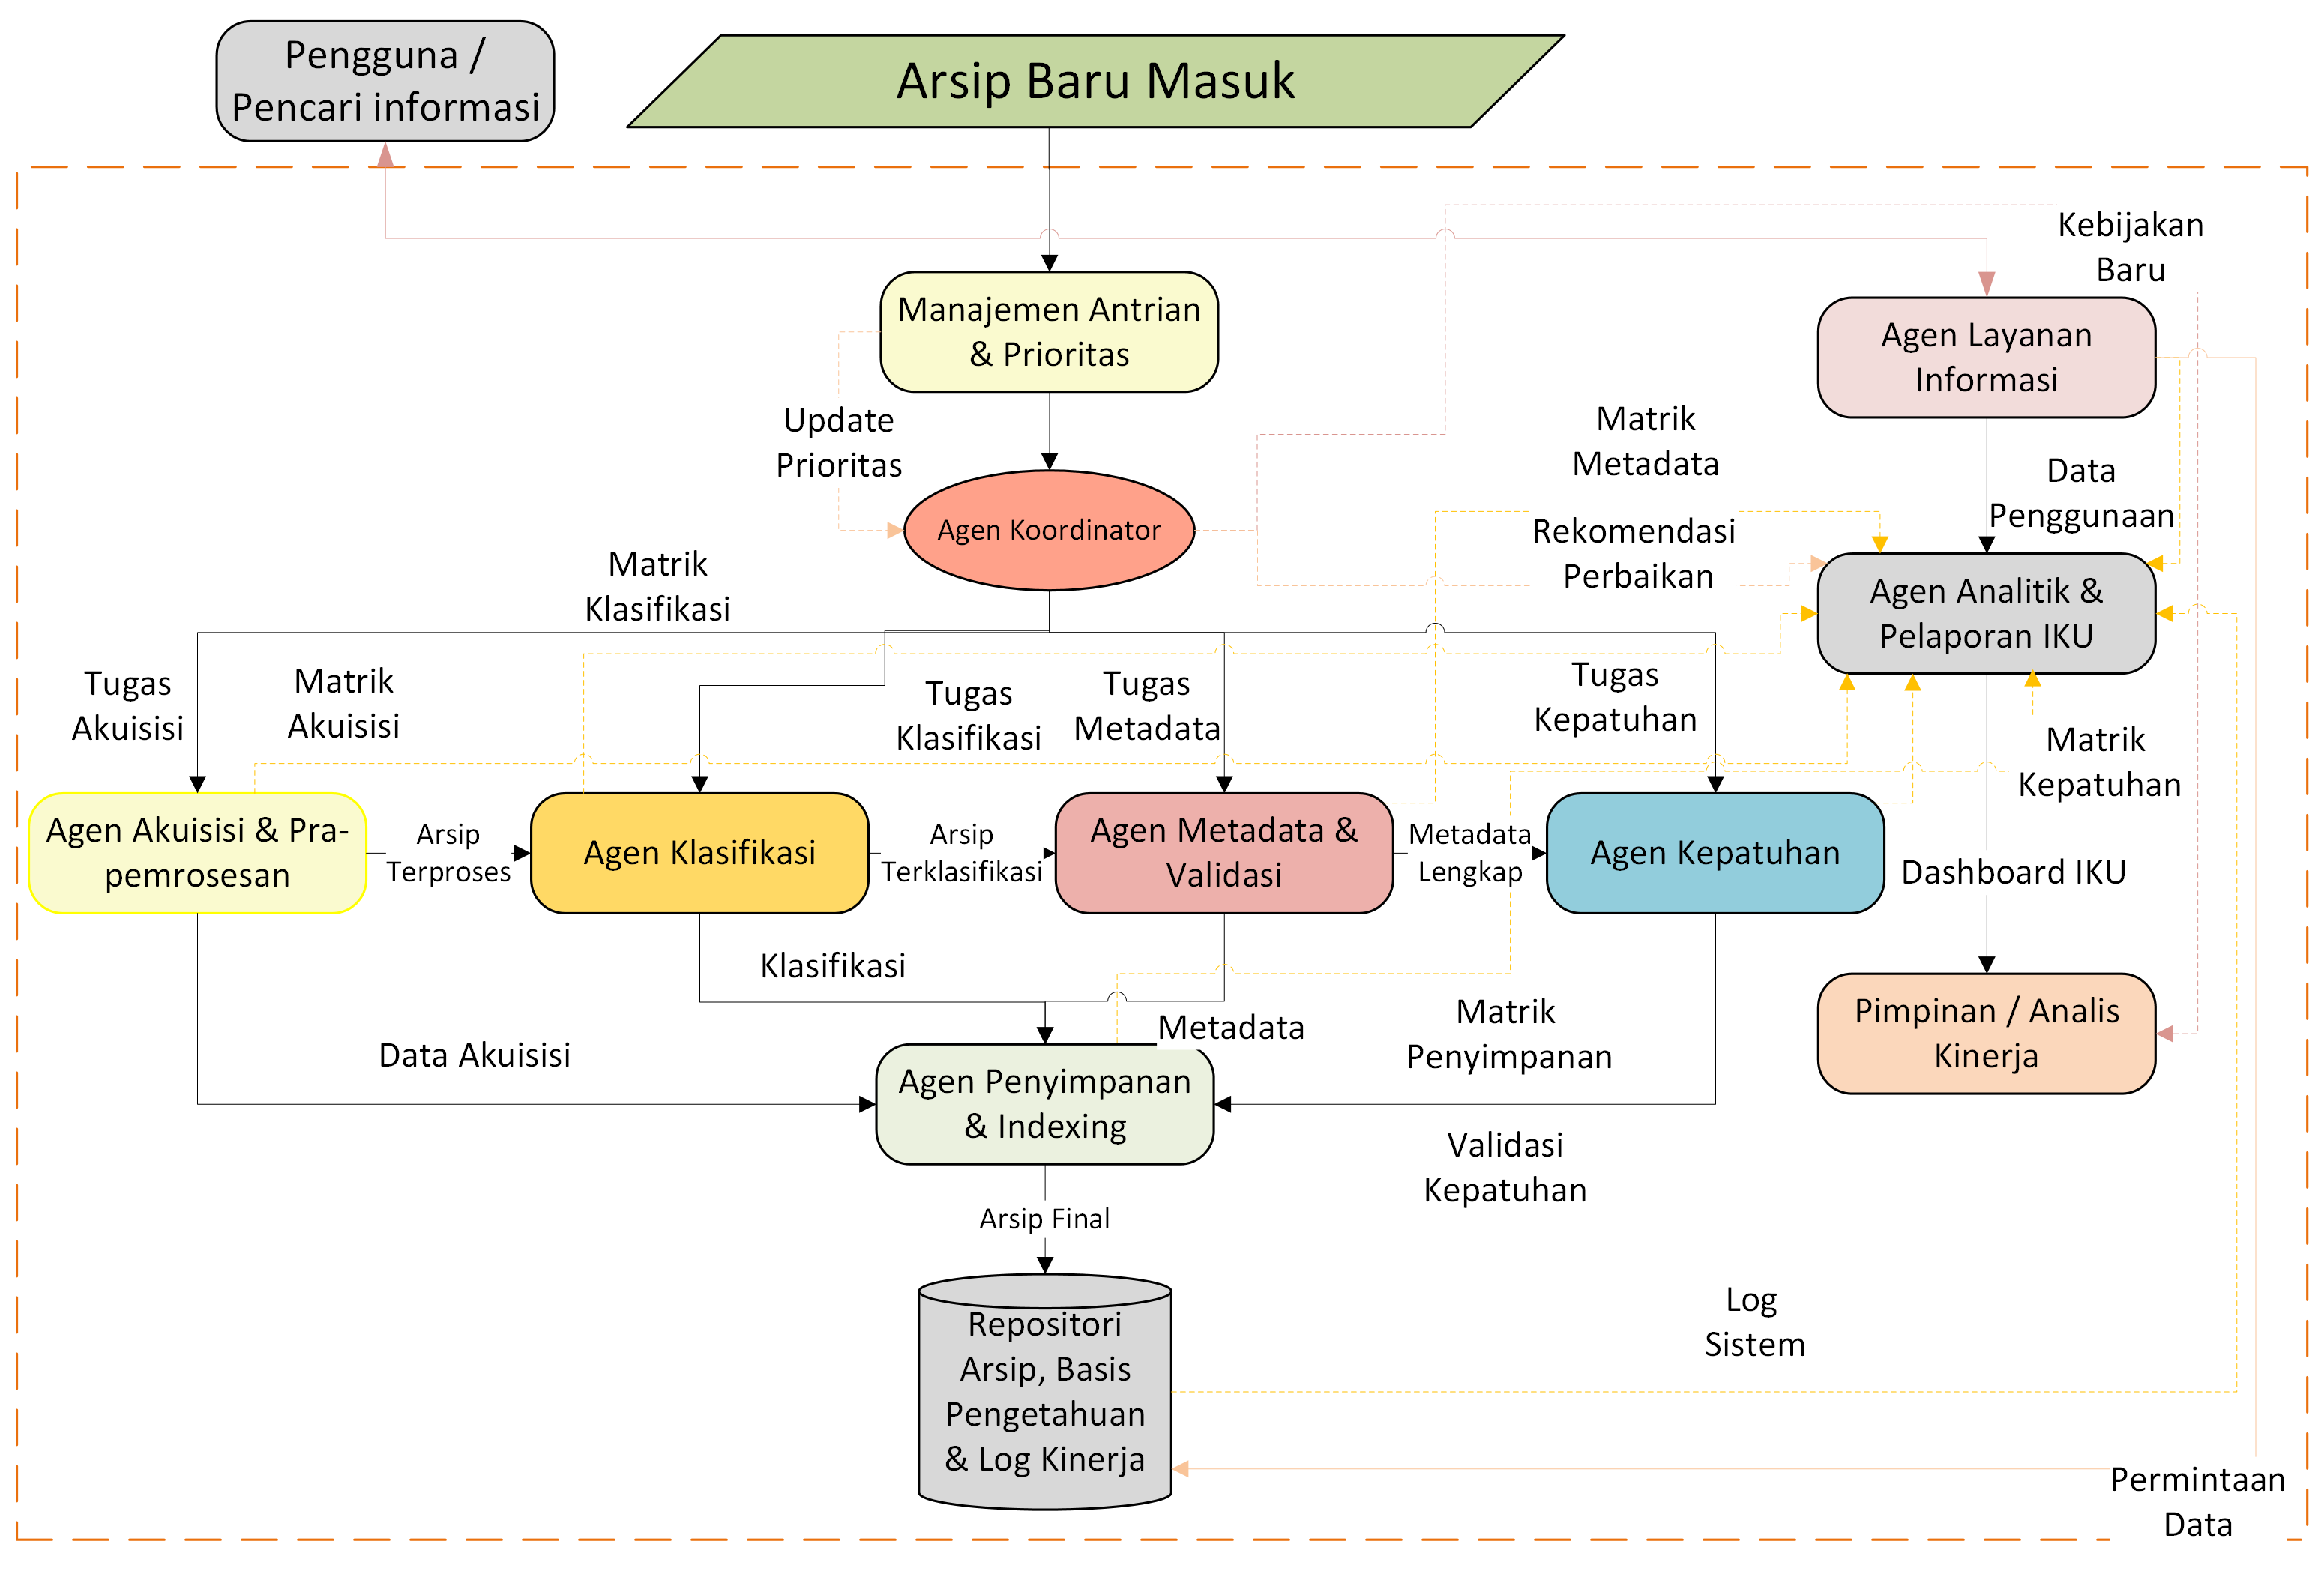
\includegraphics[width=0.8\linewidth]{media/media/image11.png}
\caption{Model Konseptual Pemanfaatan \emph{Agentic AI} dalam Tata Kelola Kearsipan}
\label{fig:model_konseptual}
\end{figure}

Meskipun alurnya otomatis, sistem ini tetap mengintegrasikan peran manusia melalui mekanisme Human-in-the-Loop (HITL) pada tahap-tahap kritis, seperti saat memvalidasi klasifikasi sensitif atau memerlukan persetujuan disposisi. Di sepanjang proses ini, setiap agen operasional secara aktif mengirimkan log aktivitas dan metrik kinerjanya ke Agen Analitik \& Pelaporan IKU, yang berfungsi untuk memantau kesehatan dan akuntabilitas sistem secara keseluruhan.

Agar seluruh alur kerja yang kompleks ini dapat berjalan secara cerdas dan konsisten, sistem bergantung pada dua fondasi utama: repositori arsip dan basis pengetahuan terpusat. Repositori arsip berfungsi sebagai tempat penyimpanan utama untuk aset digital dan informasi lokasi arsip fisik. Sementara itu, basis pengetahuan agen menjadi memori dari operasi ini, yang berisi serangkaian aturan fundamental seperti skema klasifikasi, standar metadata, JRA, serta kebijakan keamanan dan akses. Basis pengetahuan ini juga dilengkapi dengan sumber daya pendukung seperti tesaurus, model machine learning untuk agen pembelajar, dan rekam jejak sistem berupa log aktivitas yang terus diperbarui untuk memandu setiap keputusan agen.

Model arsitektur Agentic AI yang diusulkan ini menyediakan kerangka kerja untuk mendelegasikan tugas-tugas tata kelola data kearsipan kepada entitas-entitas cerdas yang dapat bekerja secara otonom, proaktif, dan terkoordinasi. Dengan mendefinisikan peran dan tanggung jawab yang jelas untuk setiap agen, serta alur kerja yang terstruktur, model ini berpotensi besar untuk meningkatkan konsistensi dalam penerapan kebijakan, meningkatkan kualitas dan struktur metadata, serta secara keseluruhan memperkuat efektivitas dan akuntabilitas tata kelola kearsipan. Keberhasilan implementasi model ini akan bergantung pada desain detail setiap agen, kualitas data dan aturan yang menjadi inputnya, serta integrasi yang cermat dengan proses bisnis dan intervensi manusia yang strategis.

\section{SIMPULAN}

Penelitian ini menyimpulkan bahwa Agentic AI, yang diimplementasikan melalui arsitektur Sistem Multi-Agen (MAS) yang terkoordinasi, memiliki potensi signifikan untuk mentransformasi tata kelola data kearsipan. Model yang diusulkan secara fundamental mengatasi tantangan terkait inkonsistensi penerapan kebijakan dan kurangnya struktur metadata yang sering terjadi pada sistem manual atau semi-otomatis. Dengan mendelegasikan tugas-tugas inti seperti akuisisi, klasifikasi, ekstraksi metadata, dan pemantauan kepatuhan kepada agen-agen cerdas yang bekerja secara otonom dan proaktif, organisasi dapat mencapai tingkat konsistensi, akurasi, dan efisiensi yang lebih tinggi dalam pengelolaan arsip.

Selain solusi teknis, penelitian ini juga mengkaji tentang pergeseran paradigma dalam tata kelola itu sendiri: dari kebijakan pasif menjadi logika aktif yang terintegrasi. Dalam model ini, basis aturan atau basis pengetahuan yang memuat skema klasifikasi, standar metadata, dan JRA tidak lagi berfungsi sebagai dokumen rujukan, melainkan sebagai komponen operasional yang secara langsung mengarahkan tindakan agen-agen AI. Agen seperti Agen Klasifikasi dan Agen Kepatuhan secara konsisten mengeksekusi aturan-aturan ini, memastikan kepatuhan secara desain (compliance by design) dan secara efektif meminimalkan risiko yang timbul dari interpretasi manusia yang berbeda atau human error.

Sebagai hasil dari transformasi tata kelola ini, implementasi Agentic AI diproyeksikan memberikan kontribusi positif dan terukur terhadap pencapaian IKU kearsipan. Peningkatan IKU ini mencakup: (a) Ketersediaan dan Aksesibilitas Arsip: Melalui otomasi proses pengolahan dan indexing yang mempercepat waktu temu kembali informasi. (b) Kualitas Metadata: Dengan otomatisasi ekstraksi, validasi kelengkapan, dan standardisasi metadata yang menjadi tulang punggung sistem kearsipan yang andal. (c) Efisiensi Layanan dan Kepatuhan: Melalui agen layanan cerdas yang merespons permintaan rutin dan agen kepatuhan yang secara proaktif memantau siklus hidup arsip sesuai regulasi.

\section{REKOMENDASI}

Berdasarkan kesimpulan di atas, dirumuskan saran untuk pengembangan penelitian selanjutnya dan rekomendasi praktis bagi institusi kearsipan.

Saran untuk Penelitian Selanjutnya: (a) Pengembangan Prototipe Fungsional: Membangun prototipe dari arsitektur MAS yang diusulkan untuk melakukan pengujian empiris terhadap kinerjanya, di luar cakupan penelitian konseptual ini. Evaluasi dapat difokuskan pada metrik seperti akurasi klasifikasi otomatis dan efisiensi alur kerja antar agen. (b) Implementasi Studi Kasus: Menerapkan model pada lingkungan institusi kearsipan nyata untuk mengidentifikasi faktor-faktor kontekstual, tantangan implementasi praktis, dan dampak organisasional secara mendalam. (c) Analisis Biaya-Manfaat: Melakukan analisis biaya-manfaat yang komprehensif untuk mengkaji nilai investasi teknologi Agentic AI, dengan membandingkan biaya implementasi terhadap keuntungan berupa efisiensi operasional, pengurangan risiko, dan peningkatan kualitas layanan.

Saran Praktis bagi Institusi Kearsipan: (a) Adopsi Paradigma Tata Kelola sebagai Logika Aktif: Institusi harus memandang adopsi AI bukan sekadar proyek otomatisasi tugas, melainkan sebagai kesempatan strategis untuk mengoperasionalkan tata kelola. Langkah awal yang krusial adalah memformalkan seluruh kebijakan dan aturan kearsipan menjadi format terstruktur yang dapat dieksekusi oleh sistem. (b) Memulai dari Skala Kecil (Pilot Project): Mengimplementasikan solusi secara bertahap. Fokus pada satu atau dua area yang paling mendesak dan berdampak tinggi, seperti otomatisasi ekstraksi metadata untuk mengurangi backlog atau pemantauan JRA untuk mitigasi risiko. (c) Pembangunan Kapasitas SDM: Mempersiapkan arsiparis dan pegawai untuk beradaptasi dengan peran baru. Pelatihan harus difokuskan untuk mengubah peran dari pelaksana manual menjadi supervisor sistem, validator dalam skema HITL, dan analis data kinerja kearsipan.

\section*{PERNYATAAN TERIMA KASIH}

Terima kasih kepada semua pihak yang telah mendukung penelitian ini.

\section*{DAFTAR PUSTAKA}

Maurel, Dominique and Nicholas Zwarich. 2021. ``Information Governance and Power Relations: Reflections on Archival Education in Québec.'' \emph{Education for Information} 37(1):33--51. https://doi.org/10.3233/efi-190360

Luo, W. and H. Hu. 2022. ``Analysis of the Path of Utilizing Big Data to Innovate Archive Management Mode to Enhance Service Capability.'' \emph{Wireless Communications and Mobile Computing} 2022:1--11. https://doi.org/10.1155/2022/6207054

Tummers, Jarno, Ayalew Kassahun, and Bedir Tekinerdogan. 2020. ``Reference Architecture Design for Farm Management Information Systems: A Multi-Case Study Approach.'' \emph{Precision Agriculture} 22(1):22--50. https://doi.org/10.1007/s11119-020-09728-0

Christiana, Nining, Siti Helminasari, and Putu Yudi Pratama. 2024. ``Technology-Driven Archival Management in Samarinda's Library Service.'' \emph{Indonesian Journal of Public Policy Review} 25(3). https://doi.org/10.21070/ijppr.v25i3.1401

Kerpedzhiev, Georgi D., Ulrich M. König, Maximilian Röglinger, and Michael Rosemann. 2020. ``An Exploration into Future Business Process Management Capabilities in View of Digitalization.'' \emph{Business \& Information Systems Engineering} 63(2):83--96. https://doi.org/10.1007/s12599-020-00637-0

Colavizza, Giovanni, Tobias Blanke, Charles Jeurgens, and Julia Noordegraaf. 2021. ``Archives and AI: An Overview of Current Debates and Future Perspectives.'' \emph{Journal on Computing and Cultural Heritage} 15(1):1--15. https://doi.org/10.1145/3479010

Ma, Ning. 2024. ``Research on Archival Data Management in Local Universities under the Context of Educational Informatization 2.0.'' \emph{Philosophy and Social Science} 1(4):95--99. https://doi.org/10.54097/wxdsk683

Liu, Zixuan. 2024. ``The Prospects and Challenges of Artificial Intelligence Technology in Archival Management.'' \emph{Academic Journal of Management and Social Sciences} 6(3):64--66. https://doi.org/10.54097/wxdsk683

Miller, John, Beth Davis-Sramek, Brian S. Fugate, Mark Pagell, and Barbara B. Flynn. 2020. ``Editorial Commentary: Addressing Confusion in the Diffusion of Archival Data Research.'' \emph{Journal of Supply Chain Management} 57(3):130--146. https://doi.org/10.1111/jscm.12236

Magnuson, John A., Rebecca Merrick, and Joseph T. Case. 2020. ``Public Health Information Standards.'' Pp. 129--145 in \emph{Health Informatics}. Springer International Publishing. https://doi.org/10.1007/978-3-030-41215-9\_8

Jones, Shawn M., Martin Klein, Michele C. Weigle, and Michael L. Nelson. 2023. ``Summarizing Web Archive Corpora via Social Media Storytelling by Automatically Selecting and Visualizing Exemplars.'' \emph{ACM Transactions on the Web} 18(1):1--48. https://doi.org/10.1145/3606030

Indrasweri, Novi, Evi Rosfiantika Dwi Wahyuni, and Rini Rakhmawati. 2022. ``Accessibility of Archival Reference Services.'' \emph{Record and Library Journal} 8(2):199--206. https://doi.org/10.20473/rlj.v8-i2.2022.199-206

Massihi, Niloofar, Neda Abdolvand, and Sahar Rajaee Harandi. 2020. ``A Business Environment Analysis Model for Renewable Solar Energy.'' \emph{International Journal of Environmental Science and Technology} 18(2):401--416. https://doi.org/10.1007/s13762-020-02826-6

Tripathi, Anil Kumar, Sambit Agrawal, and R. D. Gupta. 2020. ``Cloud Enabled SDI Architecture: A Review.'' \emph{Earth Science Informatics} 13(2):211--231. https://doi.org/10.1007/s12145-020-00446-9

Hosseini, Sajjad and Hossein Seilani. 2025. ``The Role of Agentic AI in Shaping a Smart Future: A Systematic Review.'' \emph{Array} 26:100399. https://doi.org/10.1016/j.array.2025.100399

Sapkota, Ranjan, Konstantinos I. Roumeliotis, and Manoj Karkee. 2025. ``AI Agents vs. Agentic AI: A Conceptual Taxonomy, Applications and Challenges.'' arXiv preprint arXiv:2505.10468. https://doi.org/10.48550/ARXIV.2505.10468

Shinde, Gayatri, Thea Kirstein, Sohini Ghosh, and Patricia C. Franks. 2024. ``AI in Archival Science: A Systematic Review.'' arXiv preprint arXiv:2410.09086. https://doi.org/10.48550/ARXIV.2410.09086

Masimov, Orkhan and Yashar Hajiyev. 2024. ``Integration of Artificial Intelligence (AI) in Task Management Systems.'' \emph{PAHTEI-Proceedings of Azerbaijan High Technical Educational Institutions} 41(06):501--509. https://doi.org/10.36962/pahtei41062024-55

Ackerman, Lauren. 2025. ``Perceptions of Agentic AI in Organizations: Implications for Responsible AI and ROI.'' arXiv preprint arXiv:2504.11564. https://doi.org/10.48550/ARXIV.2504.11564

Raza, Shaina, Ranjan Sapkota, Manoj Karkee, and Christos Emmanouilidis. 2025. ``TRiSM for Agentic AI: A Review of Trust, Risk, and Security Management in LLM-based Agentic Multi-Agent Systems.'' arXiv preprint arXiv:2506.04133. https://doi.org/10.48550/ARXIV.2506.04133

\end{multicols}

\end{document}